\chapter{Speichersysteme}

Speichersysteme sind eine entscheidende Komponente der IT Infrastruktur eines Unternehmens. In der heutigen Zeit kann man von Speichersystemen kaum absehen, da Big Data immer an Wichtigkeit gewinnt. Sie bieten eine Möglichkeit, große Mengen an Daten zu speichern und zu verwalten, um den Zugriff und die Nutzung zu erleichtern. Es gibt eine Vielzahl an Speichersystemen, die für verschiedene Zwecke konzipiert sind. Durch die große Auswahl in der IT und die stetig anwachsende Innovation stellt sich die Frage, welche Speichersysteme sich für bestimmte Zwecke (Use Cases) eignen. Die Wahl des richtigen Speichersystems hängt von den Anforderungen des Unternehmens ab, wie zum Beispiel der Art der zu speichernden Daten, dem benötigten Zugriff und die Skalierbarkeit. Eine gründliche Analyse der Anforderungen und Kosten ist entscheidend, um die beste Lösung zu finden, die den Bedürfnissen des Unternehmens entspricht.\\
\\ 
Im nachfolgenden Kapitel werden die unterschiedlichen Typen von Speichersystemen vorgestellt, wobei der Fokus auf den drei Speicherarten File-, Object- und Block Storage liegt. Im Anschluss daran erfolgt ein Vergleich von zwei Cloud-Providern in Bezug auf sicherer Speicherung, Hochverfügbarkeit, Performance, Kosten, API-Anbindung sowie der Dateibereitstellung. Auf Basis dieser Kriterien wird eine Entscheidung darüber getroffen, welcher Provider den Bedürfnissen von "Leoticket" entspricht. Hierbei fließen die Kosten- und Performance-Analysen mit in die Entscheidung ein.

\newpage

\section{Arten von Speichersystemen}

Im folgenden Abschnitt werden die verschiedenen Arten von Speichersystemen vorgestellt, die für die Speicherung von digitalen Daten verwendet werden. Hierbei werden die drei gängigsten Speicherarten File-, Object-, und Blob Storage behandelt.\\
 
Die heutige IT-Landschaft bietet eine Vielzahl von Speichersystemen, die je nach Bedarf und Anforderungen ausgewählt werden können. Neben den traditionellen Speichermedien wie Festplatten und Bandlaufwerken gibt es heute auch verschiedene Arten von Speichersystemen, die in der Cloud oder als lokale Lösungen bereitgestellt werden können. Dazu gehören unter anderem File Storage, Object Storage und Blob Storage.\\

Jeder dieser Speicherarten hat ihre spezifischen Vor- und Nachteile und ist für bestimmte Anwendungsfälle besser geeignet als andere. 

\newpage
 
\subsection{File Storage}

File Storage, auch dateiebenen- oder dateibasierter Storage genannt \cite{redHat-storage}, ist eine Speicherlösung bei der Dateien auf einem Dateisystem gespeichert werden. 

\begin{quote}
	Dieses System wird auch als hierarchischer Storage bezeichnet und gilt als das älteste und am weitesten verbreitete Datenspeichersystem für Direct und Network-Attached Storage. Dateisysteme organisieren Daten in hierarchischen Ordnern und Unterverzeichnissen, ähnlich wie in einem Dateiordner auf einem Computer. Dateien werden in der Regel auf einem Server oder einer Festplatte gespeichert und können von mehreren Benutzern gleichzeitig gelesen und geschrieben werden. Hierbei werden die Informationen in einzelnen Verzeichnisse abgelegt und können über den entsprechenden Pfad aufgerufen werden. Um dies zu ermöglichen, werden begrenzte Mengen an Metadaten genutzt, die dem System den genauen Standort der Dateien mitteilen, vgl. \citeauthor{redHat-storage}.
\end{quote}

In der folgenden Abbildung wird die hierarchische Struktur des Dateispeichers visualisiert.

\begin{figure}[h]
\centering
	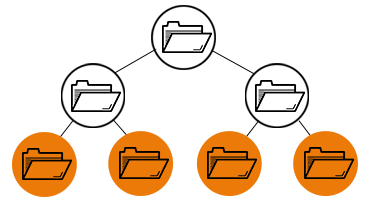
\includegraphics{Pictures/FileStorageHierarchy.png}
	\caption{File Storage: Aufbau des Hierarchiesystems, \citeauthor{redHat-storage}}
\end{figure}

File Storage wird häufig in Unternehmen und Organisationen eingesetzt, um gemeinsame Dateiserver bereitzustellen oder Daten in Cloud-Speicherdiensten wie Dropbox oder Google Drive zu speichern.
Auch wenn es von Betriebssystemen und Anwendungen gut unterstützt wird, kann die Performance und Skalierbarkeit von File Storage bei sehr großen Dateisystemen beeinträchtigt werden, was insbesondere bei stark frequentierten Anwendungen oder bei der Verarbeitung großer Datenmengen zum Problem werden kann. 

\begin{quote}
	Mit zunehmenden Datenvolumen erfordert das Skalieren von Dateispeichern das Hinzufügen neuer Hardwaregeräte oder den Austausch vorhandener Geräte durch solche mit höherer Kapazität. Dies kann im Laufe der Zeit teuer werden. \glqq As data volumes expand, scaling file storage requires [...]\grqq, (\cite{nx-fileScala}, Übersetzung des Autors)
\end{quote}

Laut Wahlmann (\citeyear{nx-fileScala}, Übersetzung des Autors) wird die Datenspeicherung bei zu vielen Daten nicht nur teuer, sondern auch unhandlich und zeitaufwändig. Der schnelle und einfache Zugriff auf jede einzelne Datei wird schwierig, wenn man zig Millionen von Dateien in Tausenden von Verzeichnissen auf Hunderten von Speichergrößen speichert. 

\newpage

\subsection{Block Storage}

Block Storage, auch genannt als Block-level Storage speichert Dateien auf SAN(Storage Area Networks) basierten Netzwerken oder auf Cloud-basierten Speicherumgebungen. Das System teilt Daten in Blöcke auf und speichert die separaten Teile jeweils mit einer eindeutigen Kennung, vgl. \cite{ibm-topics}.\\

Daten werden in Blöcken auf dem Datenträger gespeichert, die unabhängig voneinander adressiert werden können. Jeder Block ist eine feste Größe, typischerweise im Bereich von einigen Kilobytes bis hin zu einigen Megabytes. Diese Blöcke können im System an jeder Stelle gespeichert werden.

\begin{quote}
	Wenn auf Block Storage gespeicherte Daten abgerufen werden, verwendet das Server-Betriebssystem die eindeutige Adresse, um die Blöcke wieder zusammenzufügen und so die Datei zu erstellen. Der Vorteil besteht darin, dass das System nicht durch Verzeichnisse und Dateihierarchien navigieren muss, um auf die Datenblöcke zuzugreifen. Dadurch werden Effizienzen erzielt, da der Abruf von Daten schneller erfolgen kann, vgl. \cite{ibm-storage}.
\end{quote}

Typische Anwendungsbereiche des Block Storage sind Datenbanken, Virtualisierungsumgebungen und Anwendungen für Big Data-Analysen. Speicherung von strukturierten Daten wie Datenbanken, Virtuelle Maschinen und Betriebssysteme eignen sich besonders bei der Verwendung von Block Storage. Diese Art von Daten erfordert schnellen und direkten Zugriff auf bestimmte Bereiche des Speichers und muss häufig in Echtzeit ausgeführt werden. Block Storage eignet sich daher am besten für Anwendungen mit hohen Anforderungen an die Leistung und niedriger Latenzzeit.

\newpage

\subsection{Object Storage}

Object Storage hat sich als Speichertechnologie in den letzten Jahren immer stärker etabliert und wird von vielen Unternehmen als Alternative zu traditionellen Speicherlösungen wie Block- oder File Storage angesehen. Die ersten Object Storage Systeme wurden bereits in den 1990er Jahren entwickelt, aber erst mit dem Aufkommen von Big Data, IoT und der Cloud-Nutzung 
 hat es einen breiteren Einsatz gefunden. Heute bieten viele Cloud Provider wie Amazon Web Services (AWS) und Google Cloud Platform (GCP) Object Storage als einen ihrer Haupt-Cloud-Services an.
 
\begin{quote}
	Object Storage ist für den Umgang mit großen Datenvolumen und unstrukturierten Daten entwickelt wurden. Sie speichert Daten als eigenständige Objekte, die aus Daten und Metadaten bestehen und einen eindeutigen Identifier (UID) haben (\glqq Object storage (aka object-based storage) is a type of data storage used to [...]\grqq, \cite{dataCore-OS}, Übersetzung des Autors).
\end{quote}

Im Gegensatz zu hierarchischen Systemen wie beim File Storage ist das Speichersystem flach strukturiert. Durch die einfache API Anbindung kann es mit vorhandenen Anwendungen integriert werden. Nutzer können detaillierte Informationen wie beispielsweise Erstellerangaben, Schlüsselwörter sowie Sicherheit-und Datenschutzrichtlinien hinterlegen. Diese Daten bezeichnet man als Metadaten.\\

Laut \citeauthor{nx-fileScala}, 2022 ist Skalierbarkeit der Hauptvorteil, da bei der Speicherung von Petabyte und Exabyte alle Objekte in einem Namespace abgelegt werden. Selbst wenn dieser Namespace auf Hunderte von Hardwaregeräten und Standorten verteilt ist, können alle Objekte schnell abgerufen werden. Andere Vorteile von Objekt Storage beinhalten die Datenintegritätsprüfung, im Englischen bekannt als \glqq erasure coding\grqq und die Datenanalyse.\\

Auch Object Storage hat seine Nachteile. Laut \citeauthor{redHat-storage} muss das Objekt nach der Speicherung bei Veränderung komplett neu überschrieben werden. Sie sind für traditionelle Datenbanken nicht geeignet, da das Schreiben von Objekten Zeit beansprucht und man sich mit der API auseinandersetzen muss, vgl. \citeauthor{redHat-storage}.\\

Insgesamt bietet Object Storage eine skalierbare und flexible Methode zur Speicherung von unstrukturierten Daten. Organisationen sollten jedoch die Vor- und Nachteile von Object Storage im Kontext ihrer spezifischen Anwendungsfälle abwägen, um eine fundierte Entscheidung über die beste Speichermethode zu treffen.\\

%TODO Object Storage Entscheidung

Da leoticket Daten wie Rechnungen und Tickets als Dateien speichern und abrufen abruft, ist Object Storage die richtige Speicherart. 

Für leoticket ist die Object Storage Variante die am Besten geeignetste Speicherlösung, da ... %TODO Satz weiterschreiben

\newpage

\section{Aktuelle Speichertechnologien im Markt}

Die beiden größten Cloud-Speicheranbieter, Amazon Web Services (AWS) und Google Cloud Platform (GCP), bieten eine Vielzahl von Speicherlösungen an, die auf die Bedürfnisse von Unternehmen zugeschnitten sind.\\ 

In diesem Kapitel werden die aktuellen Speichertechnologien auf dem Markt untersucht, wobei der Fokus auf den Angeboten von AWS und GCP liegt. Um eine Vergleichsgrundlage zwischen AWS und GCP zu schaffen, werden die verschiedenen Aspekte wie sichere Speicherung, Hochverfügbarkeit, Leistung, Kosten, API Anbindung und die Bereitstellung der Dateien betrachtet. Dieses Vorgehen dient dazu, zu ermitteln, welche Speicherart sich am besten für welche Anforderungen eignet. Als Kontrast dazu wird das Open-Source-Objektspeichersystem MinIO betrachtet.\\

AWS bietet eine Reihe von Speicheroptionen an, darunter Amazon S3 (Simple Storage Service). Amazon S3 ist ein Object Storage-Service, der für die Speicherung und den schnellen Abruf von unstrukturierten Daten wie Videos, Fotos und Dokumenten ausgelegt ist.

Google Cloud Platform bietet ebenfalls eine Vielzahl von Speicherlösungen an, darunter Google Cloud Storage. Google Cloud Storage ist ein Object Storage-Service, der für die Speicherung von unstrukturierten Daten wie Bildern, Videos und Dokumenten ausgelegt ist.\\
 
Insgesamt bieten AWS und Google Cloud Platform eine Vielzahl von Speicherlösungen an, die auf die Bedürfnisse von Unternehmen zugeschnitten sind. Organisationen sollten jedoch die Vor- und Nachteile jeder Speicherlösung abwägen, um die beste Lösung für ihre spezifischen Anforderungen zu finden.

\newpage

\subsection{Eigenschaften}

Im vorliegenden Abschnitt werden Amazon S3 und Google Cloud Storage in Bezug auf verschiedene Kriterien untersucht. Dabei werden zunächst die Eigenschaften von AWS S3 erläutert, gefolgt von einer Betrachtung von GC Storage. Ziel ist es, die Unterschiede zwischen den beiden Anbietern hervorzuheben und eine Entscheidungshilfe zu bieten, welche Plattform für die Anforderungen von \glqq leoticket\grqq am besten geeignet ist. Die Auswahl der Kriterien erfolgt in Anlehnung an die spezifischen Anforderungen von \glqq leoticket\grqq.

%TODO Aws und GCP Definition?

\newpage

\subsubsection{Sichere Speicherung}

Viele Anbieter von Object Storage-Lösungen bieten integrierte Verschlüsselungsmöglichkeiten an, um sicherzustellen, dass Daten sowohl in Ruhe als auch in Bewegung geschützt sind. Dabei können unterschiedliche Verschlüsselungsmethoden zum Einsatz kommen. In Bezug auf die sichere Speicherung bieten sowohl AWS als auch GCP verschiedene Optionen für die Verschlüsselung von Daten.Die Sicherheit der gespeicherten Daten ist von entscheidender Bedeutung, um die Integrität und Vertraulichkeit der Daten zu gewährleisten.\\

\textbf{Amazon S3}\\

In diesem Unterabschnitt werden die verschiedenen Sicherheitsfunktionen von Amazon S3 untersucht.\\

IAM (Identity and Access Management) ist ein wichtiger Bestandteil von AWS und ermöglicht es Benutzern, Gruppen und Rollen zu erstellen, um den Zugriff auf S3 zu verwalten. Benutzer können individuelle Berechtigungen zugewiesen werden, während Gruppen und Rollen mehrere Benutzer mit denselben Berechtigungen zusammenfassen können. Auf S3-Buckets und Objekte kann man eine granuläre Zugriffssteuerung anwenden. Benutzer, Gruppen oder Rollen können so berechtigt werden, den Zugriff auf bestimmte Buckets und Objekte zu beschränken oder zu erlauben. "Beim Erteilen von Berechtigungen in Amazon S3 entscheiden Sie [...]."\cite{aws-iam-s3}\\

Eine weitere wichtige Sicherheitsfunktion von Amazon S3 ist die Datenverschlüsselung. S3 bietet eine Vielzahl von Verschlüsselungsoptionen für die serverseitige und clientseitige Verschlüsselung. Da für leoticket die clientseitige Verschlüsselung nicht in Frage kommt, liegt der Fokus auf der serverseitigen Verschlüsselung. Es gibt drei Methoden, darunter die serverseitige Verschlüsselung mit Amazon S3-verwalteten Schlüsseln (SSE-S3), mit KMS-verwalteten Schlüsseln (SSE-KMS) und die SSE-C. Diese Optionen ermöglichen es Benutzern, die Verschlüsselung auf ihre spezifischen Anforderungen abzustimmen und so die Sicherheit der Daten zu gewährleisten.

Laut \citeauthor{aws-iam-s3} nutzen Buckets standardmäßig die SSE-S3 Methode. Für die Verschlüsselung wird die 256-bit Advanced Encryption Standard (AES-256) verwendet. Seit dem 5. Januar 2023 sind alle neu erstellen Buckets auf SSE-S3 ausgelegt. Alle neuen Objekte sind beim Hochladen automatisch verschlüsselt, ohne weitere Zusatzkosten und keine Einbußung der Leistung.

\begin{quote}
	Die Serverseitige Verschlüsselung schützt die Daten at rest. Amazon S3 verschlüsselt jedes Objekt mit einem eindeutigen Schlüssel. Als zusätzliche Sicherheitsmaßnahme werden diese eindeutigen Schlüssel mit einem weiteren Schlüssel verschlüsselt, welches in regelmäßigen Abständen rotiert wird, vgl. \cite{aws-iam-s3}
\end{quote}

Amazon S3 stellt auch die SSE-KMS als Auswahl zur Verfügung. AWS-KMS ist ein Dienst, dass einen Schlüsselverwaltungssystem zur Verfügung stellt. Es verschlüsselt die Objekt Daten und speichert die S3 Checksum, das im Objekt Metadaten steckt, in verschlüsselter Form. Man kann die SSE-KMS in der AWS Management Konsole oder über die AWS KMS API verwalten. Jedoch gibt es zusätzliche Kosten bei der Verwendung der Methode. Dazu mehr im Kosten Abschnitt. Bei der Nutzung von AWS-SSE gibt es zwei Methoden. Einmal die AWS managed key oder die customer managed key. Es unterstützt die \glqq envelope encryption\grqq. Das bedeutet, das die Schlüssel für die Daten durch einen Master Key verschlüsselt wird. Dies erleichtert die Verwaltung der Schlüssel.\\

Bei der AWS managed key Variante wird automatisch ein Schlüssel erstellt, sobald ein Objekt in ein Bucket hochgeladen wird. Dieser generierte Schlüssel wird dann für die Ver- und Entschlüsselung der Daten verwendet. Wenn man einen eigenen Schlüssel bei KMS verwenden möchte, dann erstellt man zuerst einen symmetrischen Key vor der KMS Konfiguration. Bei der Bucket Erstellung kann man anschließend den selbst-erstellten Key angeben. Die Nutzung von Customer Managed Keys hat einige Vorteile, die den Anforderungen von leoticket entspricht. Selbsterstellte Schlüssel bieten mehr Flexibilität und Kontrolle. Man kann sie selber erstellen, rotieren und deaktivieren. Hinzufügend kann man auch Zugriffskontrollen und Auditierung für den Schutz der Daten konfigurieren.\\

Wenn man die SSE-KMS Variante aussucht, kann man auch die S3 Bucket Key Funktion aktivieren. Dies kann die Request Kosten bis zu 99 Prozent reduzieren, indem die Request Traffic von Amazon S3 zu AWS KMS reduziert wird. Durch die Aktivierung der S3 Bucket Key für einen Bucket werden unique data keys für die Objekte im Bucket erstellt. Diese Bucket Keys werden für eine bestimmte Zeit verwendet, welches Abrufe zu Amazon S3 nach AWS KMS reduziert um Verschlüsselungsoperationen durchzuführen.\\

Zuletzt gibt es noch die SSE-C (server-side encryption with customer-provided keys). Bei der SSE-C stellt der Customer seinen eigenen Schlüssel zur Verfügung. Dieser Schlüssel wird nicht von Amazon S3 gespeichert, im Gegensatz bei AWS KMS. Amazon S3 übernimmt mit dem bereitgestellten Schlüssel die Datenverschlüsselung beim Schreiben sowie die Datenentschlüsselung beim Zugriff auf Objekte. Amazon S3 entfernt anschließend den Schlüssel aus dem Speicher. Da Amazon S3 den Schlüssel nicht speichert, sepeichert er den zufällig generierten HMAC (Hash-baded Message Authentication Code) Wert vom Encryption Key um zukünftige Requests zu validieren."Note: Amazon S3 does not store the encryption key that you provide. [...]", \cite{aws-sse-c}.\\

Object Ownership ist eine weitere wichtige Sicherheitsfunktion von Amazon S3. Mit Object Ownership können Benutzer oder Gruppen die Eigentümerschaft von Objekten in S3-Buckets besitzen. Dies bedeutet, dass nur autorisierte Benutzer die Berechtigung haben, Objekte zu löschen oder zu ändern, was die Sicherheit der Daten erhöht.\glqq S3 Object Ownership ist eine Einstellung auf Amazon-S3-Bucket-Ebene, mit der Sie Zugriffskontrolllisten (ACLs) deaktivieren und das Eigentum an jedem Objekt in Ihrem Bucket übernehmen können, [...]." \cite{aws-iam-s3}\\ 

\newpage

AWS empfiehlt die ACL (Access Control List) auf Bucket-Ebenen deaktiviert zu lassen. Alle Objekte eines Buckets gehört so dem Bucket Owner. Laut \citeauthor{aws-iam-s3} verfügt Object Ownership über drei Einstellungen, mit denen man die Eigentümerschaft von Objekten steuern kann.

\begin{figure}[h]
\centering
	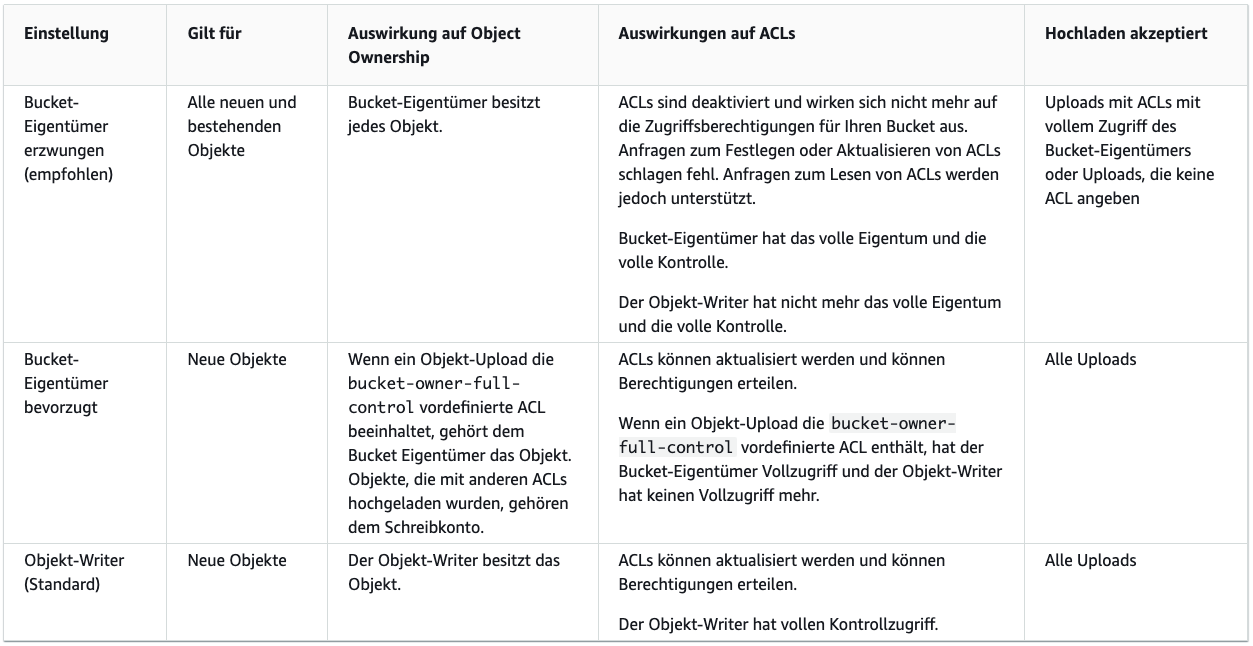
\includegraphics[width=13cm,keepaspectratio]{Pictures/objectOwnershipTable.png}
	\caption{Einstellungen für Object Ownership, \citeurl{aws-iam-s3}}
\end{figure}

Laut \citeauthor{aws-iam-s3} zeigt die obige Tabelle die Auswirkungen, die jede Einstellung für Object Ownership auf ACLs, Objekte, Objekteigentümer und Objekt-Uploads hat.\\

Logging ist ein weiterer Aspekt der Amazon S3-Sicherheit. S3 bietet verschiedene Logging-Optionen, darunter Bucket Logging und Object-Level Logging, die es Benutzern ermöglichen, Zugriffe auf S3-Objekte aufzuzeichnen und zu überwachen. Diese Funktionen sind entscheidend, um Compliance-Anforderungen zu erfüllen und verdächtige Aktivitäten zu erkennen. AWS bietet eine Vielzahl von tools zur Überwachung der Amazon S3 Ressourcen. Darunter die Amazon CloudWatch Alarms, AWS CloudTrail Logs, Amazon S3 Access Logs und die AWS Trusted Advisor.\\

%TODO compliance

\newpage

\textbf{Google Cloud Storage}\\

Auch Google Cloud bietet eine Vielzahl an Sicherheitsfunktionen, um sicherzustellen, dass Daten in der Cloud sicher gespeichert und geschützt sind. Unter anderem die Datenverschlüsselung. Google Cloud bietet genau wie Amazon S3 Serverseitige Verschlüsselung an. Hier unterscheidet man zwischen Google-managed Keys, Customer-managed encryption keys und die Customer-supplied encryption keys. Google-managed encryption ist die Standard Verschlüsselungsoption von Google Cloud. Cloud Storage verschlüsselt die Daten serverseitig, bevor die Daten auf die Festplatte geschrieben werden. 

\begin{quote}
	Die Standard Variante verwaltet für den Nutzer die Encryption Keys in ihrem eigenen Key Management System. Auch Google verwendet für die Verschlüsselung die AES-256 wie AWS. Als Nutzer muss man bei dieser Varianet keine Einstellungen berücksichtigen. Daten werden automatisch verschlüsselt beim Abruf, vgl. \cite{gcp-encrypt}.
\end{quote}

Wenn man mehr Kontrolle über die Schlüssel haben möchte, dann gibt es die Customer-managed encryption Option. Die Schlüssel werden von Cloud KMS (Cloud Key Management Service) erstellt und verwaltet. Diese Schlüssel werden vom Nutzer anschließend extern oder in einem HSM Cluster gespeichert. Customer Keys kann man für indivduelle Objekte benutzen oder einen Bucket so einstellen, dass er einen Standard Key für alle neuen Objekte verwendet. Der erstellte Schlüssel wird für die Verschlüsselung der Objektdaten, die CRC32C Checksum des Objekts und für die MD5 Hash verwendet. Als zusätzlichen Schutz gibt es die Service Agents, auch genannt als service accounts. Diesem Agent kann man bestimmte Rechte geben, sodass es Zugriff auf den gewünschten Encryption Key hat, um damit Objekte verschlüsseln zu können.\\

Zuletzt gibt es noch die Customer-supplied encryption keys. Als zusätzliche Sicherheitsebene zu Google-managed encryption keys können Nutzer ihren eigenen AES-256 Encryption Key bereitstellen, welches als Base64 encoded ist. Bei dieser Variante wird der Schlüssel nicht von Google Cloud gespeichert oder verwaltet. Die Nutzer müssen diese Schlüssel selber verwalten und speichern. Um zukünftige Requests zu validieren speichert Google Cloud einen kryptografischen Hash vom Schlüssel. Jedoch kann der Encryption Key nicht aus dem Hash regeneriert werden oder den Hash nicht zum Entschlüsseln anwenden.\\

Des weiteren gibt es auch in Google Cloud Zugriffskontrolleinstellungen, mit der Nutzer genau steuern können, wer auf ihre Daten zugreifen kann. Den Zugriff kann man auf Bucket- und Objektebene steuern und Benutzern und Gruppen bestimmte Rollen zuweisen. Dabei wird zwischen Uniform und Fine-grained unterschieden. Uniform Access Control (UAC) ermöglicht es, den Zugriff auf einen gesamten Bucket in Google Cloud Storage auf der Ebene von Rollen zuzuweisen. Dazu können verschiedene vordefinierte Rollen wie "Leser", "Schreiber" oder "Besitzer" verwendet werden, die festlegen, welche Aktionen ein Benutzer auf dem Bucket ausführen darf. UAC ist eine einfachere Methode zur Zugriffskontrolle, da die Zugriffsrechte auf Bucket-Ebene vergeben werden. Das bedeutet, dass alle Objekte in dem Bucket automatisch dieselben Zugriffsrechte haben.\\

Fine-Grained Access Control (FGAC) hingegen ermöglicht es, die Zugriffskontrolle auf die Ebene von Objekten oder sogar auf Teile von Objekten herunterzubrechen. Das bedeutet, dass jeder Benutzer oder jede Gruppe individuelle Zugriffsrechte auf bestimmte Objekte oder Teile von Objekten haben kann. Mit FGAC kann man sehr granulare Zugriffssteuerungen implementieren. Es ist eine mächtige Methode, aber auch komplexer und zeitaufwändiger zu implementieren als UAC. Mit Cloud IAM können auch rollenbasierte Zugriffssteuerungen für Bucket- unObjektebene ähnlich wie bei AWS umgesetzt werden.\\

Weitere Funktionen die Google Cloud anbietet ist Objekt Versioning, Audit Logging, Bucket Locks, VPC Service Controls, Data Loss Prevention und Identity-Aware Proxy.

\newpage

\subsubsection{Hochverfügbarkeit}

\textbf{Amazon S3}\\

Amazon S3 ist ein skalierbarer und hochverfügbarer Objekt Storage, der eine Verfügbarkeit von 99.99 Prozent garantiert.\glqq Designed to provide 99.999999999 percent durability and 99.99 percent availability of objects over a given year.\grqq, \cite{aws-availability}\\

Dies wird durch die Verwendung von Multi-Availability Zone Architekturen erreicht, die eine automatische Replikation von Daten in verschiedenen physischen Standorten ermöglichen. Die Multi-Availability Zone Architektur von Amazon S3 basiert auf der Aufteilung von Daten in mehrere geografisch getrennte Verfügbarkeitszonen (AZs). Jede AZ besteht aus mehreren physischen Rechenzentren, die sich in einem geografisch getrennten Gebiet befinden. Jede AZ ist vollständig unabhängig und bietet eine hohe Redundanz und Verfügbarkeit. Wenn ein Benutzer ein Objekt in Amazon S3 hochlädt, wird es automatisch in mehrere AZs repliziert.um sicherzustellen, dass das Objekt auch bei AUsfällen in einer AZ weiterhin verfügbar ist. Im Falle eines Ausfalls einer AZ wird Amazon S3 automatisch die Anfragen auf eine andere AZ umleiten, um eine ununterbrochene Verfügbarkeit des Objekts sicherzustellen. Durch die Cross-Region Replikation werden Daten automatisch in andere AWS-Regionen repliziert. Dadurch kann eine hohe Verfügbarkeit der Daten im Falle eines Ausfalls einer gesamten AWS-Region gewährleistet werden.\\

Amazon S3 bietet auch eine hohe Verfügbarkeit von Metadaten, die für den Zugriff auf Objekte verwendet werden. Metadaten werden automatisch in mehrere AZs repliziert, um sicherzustellen, dass die Metadaten auch im Falle eines Ausfalls einer AZ verfügbar bleiben. Zusätzlich zu Multi-Availability Zone Architekturen verwendet Amazon S3 auch Fehlerkorrektur- und Erkennungsmechanismen wie CRC-Prüfungen, um die Integrität von Daten sicherzustellen und sicherzustellen, dass die gespeicherten Daten stets korrekt sind.\\

Durch Aktivierung der Versionierung wird jeder Objektversion, die in einem Amazon S-Bucket gespeichert ist, eine eindeutige Versions-ID zugewiesen. Wenn eine Objektversion versehentlich gelöscht oder überschrieben wird, kann die vorherige Version wiederhergestellt werden.\\

Um eine hohe Verfügbarkeit bereitzustellen, stell Amazon S3 außerdem noch die S3-Transfer Acceleration zur Verfügung. Durch die Verwendung von Amazon S3-Transfer Acceleration können Benutzer die Übertragung großer Datenmengen beschleunigen, indem ein optimierter Netzwerkpfad genutzt wird. Dadurch kann de Verfügbarkeit der Daten verbessert werden, indem Verbindungsprobleme minimiert werden.\\

Um die Leistung von Amazon S3 zu überwachen und auf mögliche Probleme reagieren zu können wird CloudWatch bereitgestellt. Dadurch können Ausfallzeiten minimiert werden und herausfinden, an welchen Momenten die Verfügbarkeit am geringsten ist.

Insgesamt bietet Amazon S3 eine hochverfügbare und zuverlässige Speicherlösung, die durch Multi-Availability Zone Architekturen und Fehlerkorrekturmechanismen eine Verfügbarkeit von 99,99 Prozent gewährleistet.

\newpage

\textbf{Google Cloud Storage}\\

Laut \cite{gcp-sla} wird die Verfügbarkeit von Google Cloud Storage als Service Level Agreement (SLA) angegeben, das die garantierte Verfügbarkeit für den Dienst definiert. Gemäß dem aktuellen SLA von Google Cloud Storage beträgt die garantierte Verfügbarkeit für Multi-Regionaler Speicher 99,95 Prozent und für Regionale Speicher 99,9 Prozent. Diese Zahlen geben an, dass Google Cloud Storage darauf ausgelegt ist, eine sehr hohe Verfügbarkeit zu gewährleisten. In der folgenden Tabelle werden diese Werte nochmals belegt.

\begin{figure}[h]
	\centering
	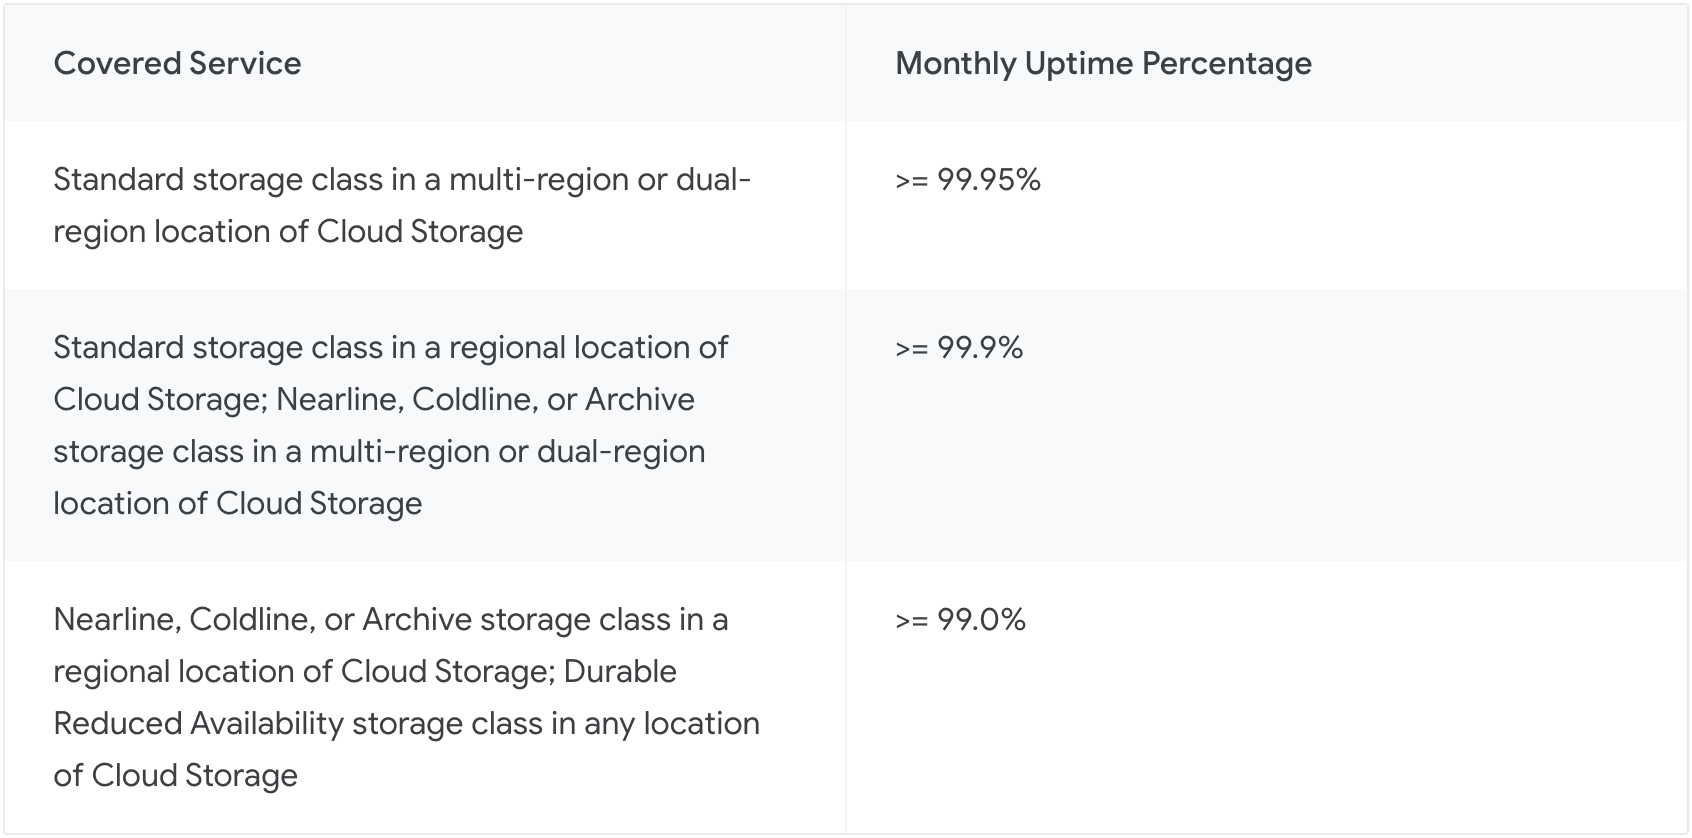
\includegraphics[width=12cm,keepaspectratio]{Pictures/GCSLA.png}
	\caption{Verfügbarkeit der Speicherklassen gemäß Google Cloud Storage SLA \citeurl{gcp-sla} }
\end{figure}

Es ist jedoch zu beachten, dass die tatsächliche Verfügbarkeit von Google Cloud Storage von mehreren Faktoren abhängt, einschließlich der spezifischen Konfiguration, dem Datenzugriffsmuster, der Netzwerkverfügbarkeit und anderen betrieblichen Variablen. Es ist daher möglich, dass die tatsächliche Verfügbarkeit in der Praxis leicht von der garantierten Verfügbarkeit abweicht.

Auch Google Cloud Storage bietet die Multi-Region Storage an. Dies ermöglicht die Speicherung von Daten in mehreren Regionen weltweit. Dadurch werden die Daten redundant repliziert und bleiben auch im Falle eines Ausfalls einer Region verfügbar.\\ 

Object Versioning bietet wie AWS die Möglichkeit Objektversionen beizubehalten. Dadurch können vorherige Versionen von Objekten wiederhergestellt werden, falls sie versehentlich gelöscht oder überschrieben werden.\\

Mit der Bucket- und Objekt Replikation können Daten automatisch in andere Regionen oder Projekte repliziert werden. Dies ermöglicht eine geografische Redundanz und verbessert die Verfügbarkeit der Daten. Google Cloud Storage verwendet verteilte Speichersysteme eine redundante Infrastruktur, um eine hohe Datensicherheit- und Verfügbarkeit zu gewährleisten. Die Daten werden in mehreren Datenzentren repliziert, um Ausfälle zu vermeiden.\\

Ein weiterer Punkt ist die Monitoring und Fehlererkennung wie Stackdriver Monitoring, um die Leistung und Verfügbarkeit von google Cloud Storage zu überwachen und auf potenzielle Probleme zu reagieren.

\newpage

\subsubsection{Kosten}

In diesem Abschnitt werden die Kosten von Amazon S3 und Google Cloud Storage betrachtet. Dabei werden die allgemeinen Kosten erläutert für welche die Cloud Provider Gebühren fordern. Bei der Kostenanalyse werden anschließend die Daten von leoticket genommen und eine grobe Abschätzung der Kosten durchgeführt.\\

Amazon S3 setzt Gebühren für die Speicherung, Anforderungen und Datenabrufe, Datenübertragung, Verwaltung und Analyse, Replikation und S3 Objekt Lambda. Für die Speicherung ist die Gebühr abhängig von der Größe der Objekte, der Speicherdauer während des Monats und der Speicherklasse. Es gibt verschiedene Speicherklassen zur Auswahl, die für verschiedenen Use Cases geeignet sind. Das wären die S3 Standard, S3 Intelligent-Tiering, S3 Standard – Infrequent Access, S3 One Zone – Infrequent Access, S3 Glacier Instant Retrieval, S3 Glacier Flexible Retrieval (früher S3 Glacier) und S3 Glacier Deep Archive. S3 Glacier wird in dieser Arbeit nicht behandelt, da leoticket keine Anwendung für diese Speicherklasse hat. Es werden die Speicherklassen S3 Standard, S3 Intelligent-Tiering, S3 Standard - Infrequent Access und S3 One Zone - Infrequent Access untersucht.

Um das Ganze zu veranschaulichen, werden die Preise durch die untere Tabelle präsentiert.

\begin{figure}[h]
	\centering
	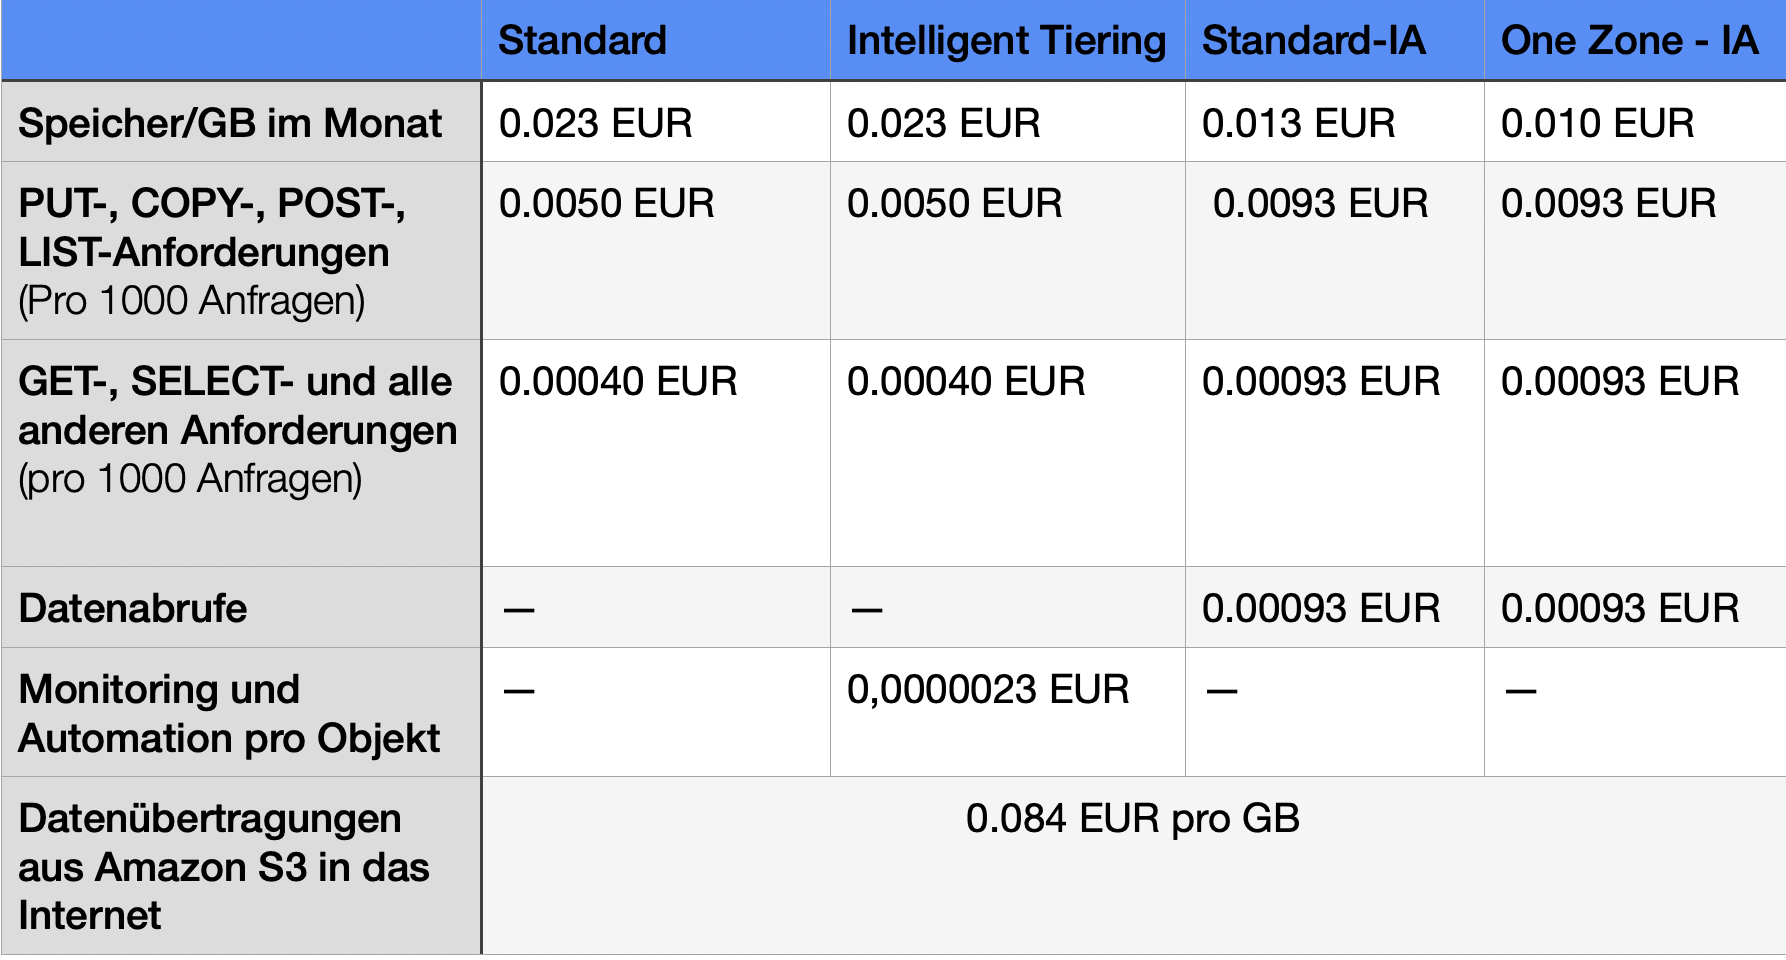
\includegraphics[width=12cm,keepaspectratio]{Pictures/AllgKostenAWS.png}
	\caption{Übersicht der Kosten der AWS S3 Speicherklassen}
\end{figure}

In der obigen Tabelle werden die Standard Preise von den verschiedenen Speicherklassen von Amazon S3 dargestellt. Die One Zone -IA hat dabei die niedrigsten kosten im Vergleich zur Standard Speicherklasse. Jedoch sind die Kosten für die Anfragen beim One zone - IA genauso wie beim Standard - IA höher als beim Standard und Intelligent Tiering. Zusätzlich werden bei Datenabrufen in den Fällen von Standard-IA und One Zone-IA Gebühren von 0.01 USD pro GB erhoben. So sind die Speicherklassen Standard und Intelligent Tiering für häufig abgerufene Daten, bei denen eine sofortige Verfügbarkeit und eine niedrige Latenzzeit erforderlich ist geeignet. Standard bietet eine hohe Leistung und ist ideal für Anwendungen, bei denen schneller Zugriff auf die Daten erforderlich ist. Die Intelligent Tiering eignet sich für Daten mit wechselndem Zugriffsverhalten. Sie analysiert das Zugriffsmuster der Objekte und verschiebt sie automatisch zwischen zwei Zugriffstiers. Dadurch kann man Kosten sparen, da man für den tatsächlichen Zugriff auf die Daten bezahlt und nicht für eine dauerhafte Speicherung in der teureren Speicherklassen.\\

Standard-IA und One Zone-IA bieten kostengünstigere Optionen für die Speicherung der Daten. Die Standard-IA ist für Daten geeignet, auf die weniger häufig zugegriffen wird, aber bei Bedarf schnell verfügbar sein müssen. Im Vergleich zur Standardklasse sind die Kosten für die Speicherung niedriger, aber es fallen zusätzliche Gebühren für den Datenabruf an. Wenn Daten von zwei Speicherklassen hergeschoben werden, dann fallen Kosten für den Speicherklassenwechsel an. Diese hängen von der Datenmenge ab, die verschoben werden.\\

Die One Zone-IA ist für Daten geeignet, auf die selten abgerufen werden, jedoch mit einer Einschränkung. Anders als bei den anderen Speicherklassen wird One Zone-IA nur in einem einzelnen Availability Zone in einer bestimmten Region gespeichert. Dies bedeutet, dass die Daten in einer einzigen AZ verfügbar sind und ein potenzieller Datenverlust auftreten kann, wenn diese AZ nicht verfügbar ist.\\

Bei der Replikation von Daten zahlt man gebühren für die Speicherung in den ausgewählten Ziel-S3-Speicherklassen, für die primäre Kopie, für Replikations-PUT Anforderungen und für anwendbare Gebühren für den Speicherabruf mit seltenem Zugriff. Laut aws preise zahlt man auch für den regionenübergreifenden Datentransfer OUT von S3 zu jeder Zielregion. Die Preise für Speicher- und PUT-Anfragen für die replizierte Kopie basieren auf den ausgewählten AWS-Zielregionen, während die Preise für Datenübertragungen zwischen den Regionen auf der AWS-Quellregion basieren. Wenn man S3 Replication Time Control nutzt, zahlt man eine Datenübertragungsgebühr für die Replikationszeitsteuerung sowie die Gebühren für S3-Replikationsmetriken, die zum selben Tarif abgerechnet werden wie angepasste Amazon-CloudWatch-Metriken. Die kosten für die S3 Replication Time Control-Datenübertragung beträgt pro GB 0.015 USD. https://aws.amazon.com/de/s3/pricing/ \\


Auch bei der Objekt Versionierung fallen Kosten an, wenn man ältere Versionen von Objekten beibehalten möchte. Die Kosten beziehen sich auf den zusätzlichen Speicherplatz, der für die Aufbewahrung der Versionen verwendet wird. Für das Tagging von benutzerdefinierten Metadaten bei Objekten selbst fallen keine direkten Kosten an. Allerdings können Kosten für das Abrufen von Tags über die S3-API(z.B. mit der ListObjects- oder GetObject-Operationen) anfallen, da dies als Datenabruf betrachtet wird und entsprechende Gebühren gemäß den AWS-Preisen Datenzugriff erhoben werden. Es ist zu beachten, dass die genauen Preise für Objektversionierung und Tagging von Amazon S3 sich im Laufe der Zeit ändern können.\\

Die genauen Preise und Kostendetails für S3 Standard IA können sich im Laufe der Zeit ändern. Es wird empfohlen, die aktuellsten Informationen auf der offiziellen AWS-Preisseite oder im AWS-Kostenrechner zu überprüfen, um eine genaue Kosteneinschätzung zu erhalten.

\newpage

\textbf{Google Cloud Storage}\\

Google Cloud Storage setzt Preise für die Komponenten Datenspeicher, Datenverarbeitung und Netzwerknutzung. Beim Datenspeicher ist wie bei Amazon S3 die Menge der in den Buckets gespeicherten Daten bedeutend. Preise für Speicher hängen von der Speicherklasse der Daten und dem Standort der Buckets ab. Bei der Datenverarbeitung werden Gebühren für die von Cloud Storage durchgeführten Verarbeitung, einschließlich Vorgangsgebühren, anwendbarer Abrufgebühren und Replikation zwischen Regionen erhoben. Bei der Netzwerknutzung werden Gebühren für die Menge der aus den Buckets gelesenen oder zwischen diesen verschobenen Daten erhoben. Google Cloud Storage bietet vier Speicherklassen an von denen drei untersucht werden. Die Standard, Nearline und Coldline. Diese drei Speicherklassen haben unterschiedliche Leistungseigenschaften und Kosten. Die Preise variieren je nach gewählter Speicherklasse.\\

Um den Vergleich zwischen Amazon S3 und Google Cloud Storage zu veranschaulichen wird eine Tabelle in der unteren Abbildung gezeigt.(siehe Abb. 2.2.3)

\begin{figure}[h]
	\centering
	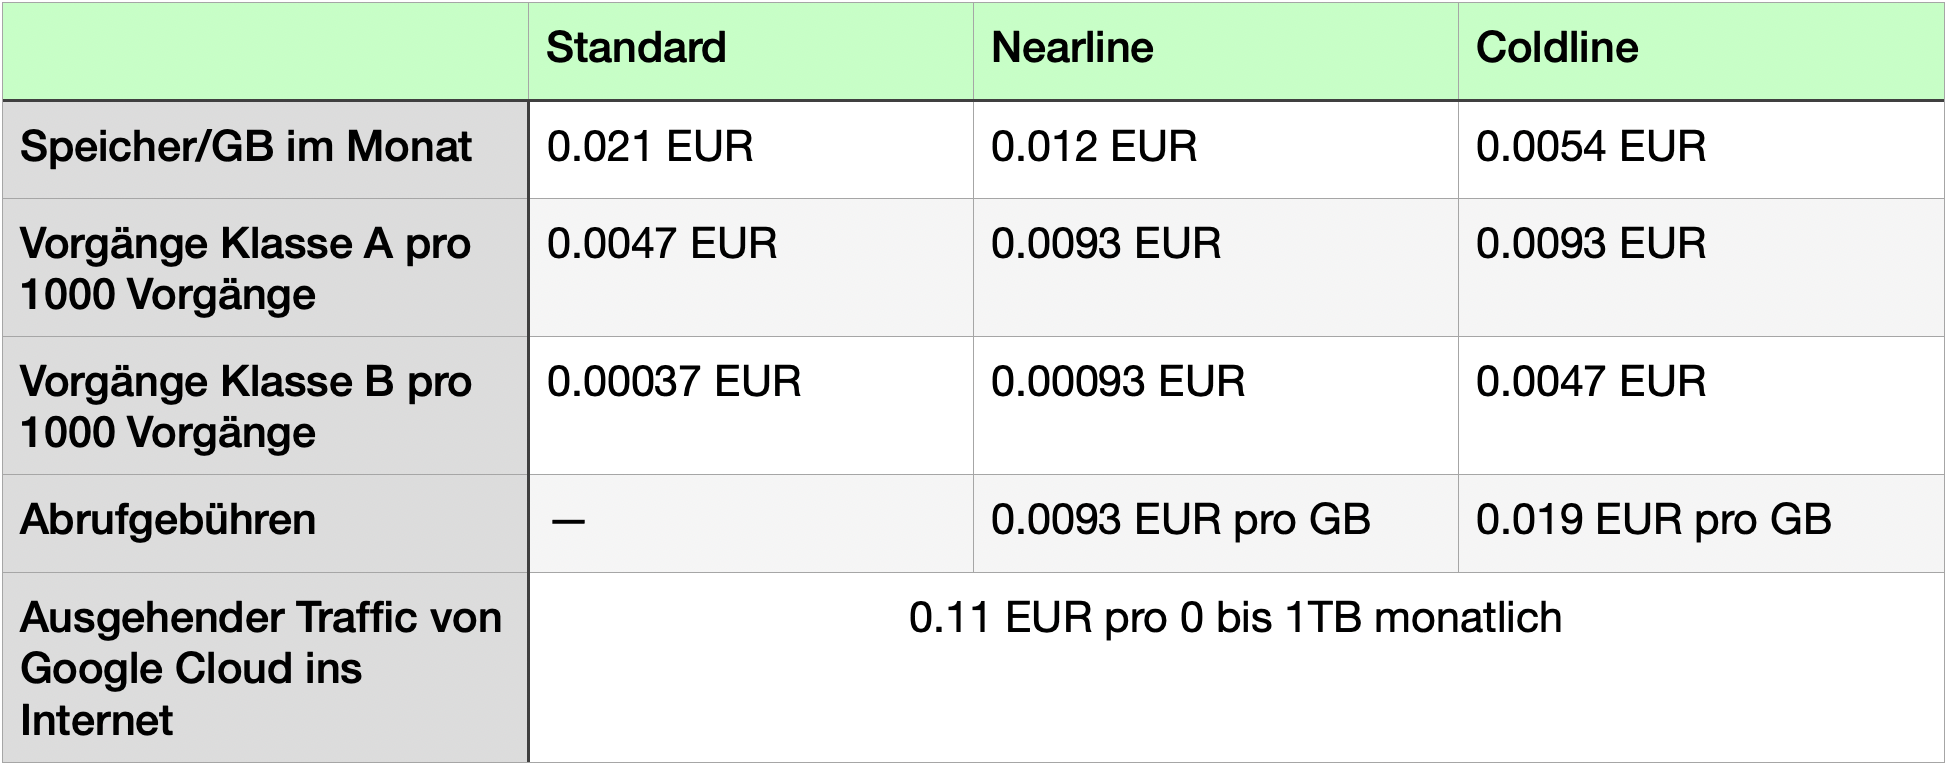
\includegraphics[width=12cm,keepaspectratio]{Pictures/GCStorageClassKosten.png}
	\caption{Vergleich der Kosten von Google Cloud Storage Speicherklassen}
\end{figure}

Ähnlich wie bei Amazon S3 sind die Speicherkosten der Nearline und Coldline geringer als die Standard Speicherklasse. Dafür werden Gebühren für die Datenabrufe bei Nearline und Coldline erhoben. Die verschiedenen Speicherklassen sind für unterschiedliche Anwendungsfälle ähnlich wie bei Amazon S3 konzipiert. Die Standard Storage-Klasse bietet hohe Performance, niedrige Latenzzeiten und hohe Verfügbarkeit. Sie eignet sich gut für häufig genutzte Daten, bei denen schneller Zugriff und gerine Latenz von Bedeutung sind. Beispiele dafür sind aktive Anwendungen, Datenbanken oder Inhalte mit hohem Durchsatz. Die Nearline Storage-Klasse ist für seltener genutzte Daten konzipiert, auf die jedoch mit niedriger Latenzzeit zugegriffen werden muss. Es bietet niedrigere Speicherkosten als die Standard Storage, jedoch mit einer etwas längeren Zugriffszeit. Es eignet sich für Backup-Daten, Archivierung und lange Speicherung. Letztere Speicherklasse, die Coldline Storage ist für Daten ausgelegt, auf die selten zugegriffen wird und bei denen eine längere Zugriffszeit akzeptabel ist. Es bietet die niedrigsten Speicherkosten an. Sie eignet sich gut für langfristige Archivierung, Compliance-Daten und Backup-Daten.\\ 

Zusätzliche Kosten, die nicht in der Tabelle aufgelistet sind, sind die Kosten für die Replikation der Daten. Auf Wunsch können Nutzer in Cloud Storage Daten innerhalb einer Region, in Dual-Regionen oder Multiregionen replizieren. Zusätzlich zu den Daten, die in den hochgeladenen Objekten enthalten sind, werden benutzerdefinierte Metadaten auf die monatliche Speichernutzung angerechnet. Für die benutzerdefinierten Metadaten "NAME:VALUE" erfasst Google Cloud Storage beispielsweise jedes Zeichen in NAME und VALUE als Byte, das mit dem Objekt gespeichert wird.\\

Beim vorzeitigen Löschen eines Objektes aus den Speicherklassen Coldline und Nearline werden Gebühren erhoben, da eine Mindestspeicherdauer angesetzt ist. Das vorzeitige Löschen beim Nearline beträgt pro GB pro Tag ca. 0.00043 USD und beim Coldline 0.0002 USD. Auch für Tags fallen Gebühren pro Monat von 0.005 USD an, dass für Buckets angehängt werden.\\

Auch hier fallen Kosten für die Objektversionierung an. Die Kosten setzen sich aus zwei Hauptkomponenten zusammen. Einmal den Speicher und die Anfragen.Jede Version eines Objekts belegt Speicherplatz im Bucket. Die kosten basieren auf der Größe der Objekte und der Anzahl der Versionen, die gespeichert sind. Das Hochladen, Herunterladen oder LÖschen von Objektversionen führt zu Anfragen an den Storage-Dienst. Für diese Anfragen können GEbühren anfallen, die sich nach der Anzahl der Anfragen richten. Es ist wichtig zu beachten, dass die Kosten für die Objektversionierung zusätzlich zu den regulären Kosten für die Speicherung und den Datenverkehr in Google Cloud Storage anfallen. Daher sollten die potenziellen Kosten der Objektversionierung in den Kalkulation einbezogen werden.

\newpage

\subsubsection{Performance}

\textbf{Amazon S3}\\

Amazon S3 bietet verschiedene Funktionen und Dienste, die die Performance und Skalierbarkeit der Datenzugriffe verbessern. In der offiziellen Dokumentation \cite{performance-guide} werden verschiedene Best Practices Guidelines empfohlen, die die Leistung erhöhen können. Es wird empfohlen HTTP Analyse Tools zu verwenden, um die Leistung von DNS lookup times, Latenzen und die Datentransfergeschwindigkeiten zu messen.\\

Eine andere Methode, die die Leistung erhöhen kann, ist die horizontale Skalierung von Connections. Da Amazon S3 als ein sehr großes verteiltes System gilt, können dadurch Requests über getrennte Verbindungen verteilt werden, um auf die maximale Bandbreite zu kommen. \glqq Amazon S3 doesn't have any limits for the number of connections made to your bucket.\grqq, \cite{performance-guide}.\\Außerdem verspricht Amazon S3, dass Requests beim wiederholten Mal wahrscheinlicher erfolgreich und schneller sind, da sie einen anderen Pfad als beim ersten Request nehmen.\glqq[...] if the first request is slow, a retried request is likely to take a different path and quickly succeed.\grqq, \cite{performance-guide}.\\

Weitere Funktionen die für die Leistungserhöhung beitragen sind die S3 Transfer Acceleration, S3 Select und die S3 Cross-Replication. Die S3 Transfer Acceleration ermöglicht schnelle, einfache und sichere Übertragungen von Dateien über große geografische Distanzen hinweg zwischen dem Client und S3 Buckets. Die Daten werden über eine optimierte Route an Amazon S3 weitergeleitet. Diese Funktion ist für Daten in Größe von Gigabytes zu Terabytes geeignet, die regelmäßig verschickt werden müssen. Um die Geschwindigkeit zu messen, bietet Amazon S3 die S3 Transfer Acceleration Speed Comparison Tool an, um beschleunigte und nicht-beschleunigte Uploads zu messen.\\

S3 Select ermöglicht das effiziente Abrufen von spezifischen Daten aus Objekten in Amazon S3. Anstatt ein gesamtes Objekt herunterladen zu müssen, können mit S3 Select nur die benötigten Daten abgefragt werden. Dies reduziert den Datenverkehr und beschleunigt den Abrufvorgang erheblich,  insbesondere bei großen Daten.\\

S3 Cross-Region Replication ermöglicht die Replikation von Daten zwischen verschiedenen AWS-Regionen. Durch die Replikation in geografisch entfernte Regionen kann die Leistung verbessert werden, indem Daten näher an den Benutzer oder Anwendungen bereitgestellt werden. Dadurch werden niedrigere Latenzzeiten und eine bessere Verfügbarkeit erzielt.\\

Die AWS SDK stellt eine einfache API und wird regelmäßig geupdatet, um die neuesten Technologien anzubieten. Die SDK beinhaltet die automatische Retry Request bei HTTP 503 Fehlern. Es beinhaltet auch den Transfer Manager, der dafür sorgt Connections automatisch horizontal zu skalieren. Damit können tausende von Requests pro Sekunde erreicht werden.

\newpage

\textbf{Google Cloud Storage}\\

Google Cloud Storage ermöglicht die Auswahl des geeigneten Speicherorts für Daten, um die Latenzzeiten zu minimieren. Man kann zwischen multi-regionalen Speicherstandorten oder regionalen Speicherstandorten wählen, um Daten näher an den Benutzer oder Anwendungen zu speichern und den Zugriff zu beschleunigen.\\ 

Durch die Integration mit Content Delivery Networks (CDNs) kann die globale Verteilung von Daten optimiert und die Bereitstellung beschleunigen. Das CDN stellt eine Zwischenspeicherung von Inhalten in Edge-Servern weltweit bereit, um den Zugriff auf Daten schneller und effizienter zu machen.\\

Bei der Performance spielt die Request Rate auch eine bedeutsame Rolle. Das bietet das Auto-Scaling von GCP an. Cloud Storage ist ein multi-tenant Service, was bedeutet, dass Benutzer die zugrunde liegenden Ressourcen gemeinsam nutzen. Um die gemeinsam genutzten Ressourcen optimal zu nutzen, haben Buckets eine anfängliche I/O Kapazität."Cloud Storage is a multi-tenant service, meaning that users share the same set of underlying resources.[...]", \cite{gcp-autoscale} (Übersetzung aus Google Cloud)

 \begin{quote}
 	Diese Kapazitäten betragen etwa 1000 Schreibzugriffsanfragen pro Sekunde für Objekte, einschließlich Hochladen, Aktualisieren und Löschen von Objekten. Es ist zu beachten, dass Cloud Storage auch eine kleinere Begrenzung für wiederholte Schreibvorgänge mit demselben Objektnamen hat. Auf Lesezugriffsanfragen po Sekunde betragen sie bei 5000, einschließlich Auflisten von Objekte, Lesen von Objektdaten und Lesen von Objektmetadaten, vgl. \cite{gcp-autoscale}.
 \end{quote}
 
 Wenn die Anfragehäufigkeit für einen bestimmten Bucket steigt, skaliert Cloud Storage automatisch und erhöht die I/O Kapazität für diesen Bucket, indem die Anfragelast auf mehrere Server verteilt wird.\\
 
Cloud Storage ermöglicht den parallelen Upload und Download von Daten, um die Übertragungs-geschwindigkeit zu maximieren. Es können mehrere Threads oder Prozesse verwenden werden, um Daten gleichzeitig hochzuladen oder herunterzuladen und so die Leistung zu verbessern.\\

Der Google Cloud Storage Transfer Service ermöglicht den schnellen und effizienten Transfer von großen Datenmengen. Daten können aus anderen Cloud-Speicherlösungen, On-Premise-Speichern oder öffentlichen Datensätzen in Google Cloud Storage übertragen werden, um Zeit und Bandbreite zu sparen.

\newpage

Während die out-of-the-box Performance bereits stabil ist, gibt es einige Einstellungen und Empfehlungen von Google Cloud, um die Performance auf den Anwendungsfall zu optimieren. Umm die Leistung messen zu können, bietet Google Cloud die "perfdiag" Tool an. Der Autor McAnlis empfiehlt in seinem Block \citetitle{gcp-blog} dieses Tool zu verwenden, dass eine Reihe von Tests durchläuft, die die aktuelle Performance von einem Cloud Bucket protokolliert. Des Weiteren empfiehlt er die Nutzung des "gsutil" Tools von Google Cloud, um kleinere Dateien schneller hochzuladen. Wenn man 20 000 Dateien, die jeweils 1kb groß sind, hochladen möchte, dann dauert der Overhead bei jedem individuellen Upload länger als die gesamte Uploadzeit gemeinsam. Deshalb sollte man Batch Operationen verwenden, da diese den Overhead reduzieren und die Leistung verbessern. Das gsutil Tool bietet die Option an Batch Operationen durchzuführen. Auf dem folgenden Diagramm wird ein Test mit 100 mal 200 000 Dateien mit individuellem Upload und Batch Upload angezeigt, das mit "gsutil -m cp" in ein Storage Bucket hochgeladen wird.

\begin{figure}[h]
	\centering
	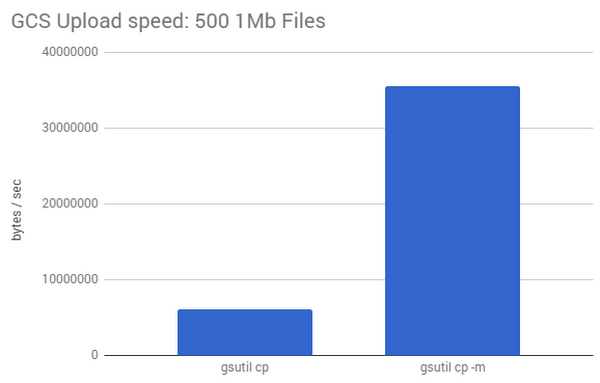
\includegraphics[width=12cm,keepaspectratio]{Pictures/cloud-storage-performance.png}
	\caption{GCS Upload Geschwindigkeit, \citeurl{gcp-blog}}
\end{figure}

Hier sieht man, wie die Leistung sich dabei um das fünffache erhöht im Gegensatz zu den inidivduellen Uploads.\\

Das Auto-balancing von Google Cloud sorgt für die Verteilung der Upload-Connections auf "Backend Shards". Das funktioniert durch die Name/Pfad der Datei und kann die Upload Geschwindigkeit erhöhen, wenn sich die Dateien in unterschiedlichen Ordnern befinden oder auch verschiedene Namensgebungen haben. Falls sich die Dateien zu sehr ähneln, kann dies die Upload Geschwindigkeit reduzieren, da die Connections alle in den gleichen Shard übergehen.\\

Eine weitere Methode, die die Performance steigern kann, sind Requests in Größe ab 1MB. Bei kleineren Requests sollte man die Requests versuchen zu parallelisieren, damit die fixen Latenzkosten überlappen.\\

Es ist zu beachten, dass die Performance auch von anderen Faktoren abhängt, wie die Anwendungsarchitektur, die Netzwerkverbindung und die Implementierung in der Anwendung. Es können spezifische Konfigurationsoptionen genutzt werden, um die Leistung weiter zu optimieren, wie Caching, asynchrone Operationen oder die Nutzung von optimierten Bibliotheken oder Frameworks. 

\newpage

\subsubsection{API Anbindung}

\textbf{Amazon S3}\\

Die API-Anbindung von Amazon S3 ist umfangreich und bietet Entwicklern eine Vielzahl von Möglichkeiten zur Interaktion mit dem Speicherdienst. Amazon S3 bietet eine RESTful API (Application Programming Interface) sowie verschiedene SDKs (Software Development Kits) und Tools, die die Integration und Nutzung erleichtern.\\

Amazon S3 bietet eine RESTful API, die auf dem HTTP-Protokoll basiert. Mit dieser API können Entwickler HTTP-Anfragen wie GET, PUT, POST und DELETE verwenden, um auf Buckets und Objekte in Amazon S3 zuzugreifen, sie zu erstellen, zu lesen, zu aktualisieren und zu löschen. Jedoch empfiehlt Amazon die Nutzung der AWS SDK, da man bei der REST API den nötigen Code für die Kalkulierung der validen Signatur schreiben muss, um sich zu authentifizieren.\glqq It requires you to write the necessary code to calculate a valid signature to authenticate your requests.\grqq, \cite{aws-api}.\\

Die AWS SDK authentifziert Requests durch die Bereitstellung der Access Keys, so fällt das Schreiben des Codes dafür weg. Die SDK ist in verschiedenen Programmiersprachen zugänglich, daruner Java, Javascript, Python, .NET, Ruby, PHP, IOS und Android. Die folgende Tabelle zeigt alle unterstützten Programmiersprachen an.

\begin{figure}[h]
\centering
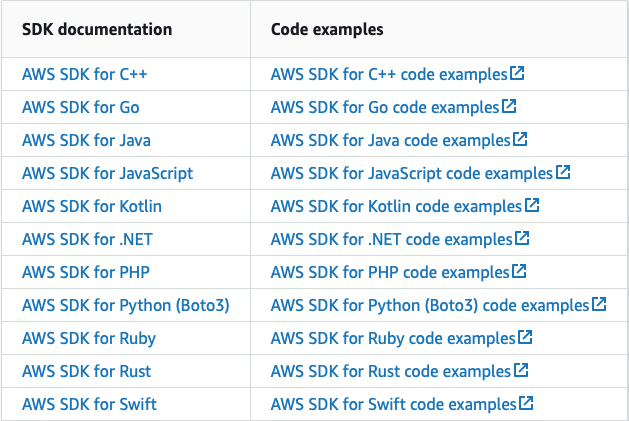
\includegraphics[width=9cm,keepaspectratio]{Pictures/SDKProgrammiersprachen.png}
	\caption{Unterstützte Programmiersprachen von AWS SDK, \citeurl{aws-sdk} }
\end{figure}

Sie bietet eine abstrakte Schnittstelle, um die Entwicklung von Anwendungen zu erleichtern und die Interaktion mit Amazon S3 zu vereinfachen. Darüber hinaus gibt es auch Drittanbieter-Tools und Open-Source Bibliotheken, die die Integration mit Amazon S3 unterstützen. Spring Boot stellt eine Bibliothek für die alte und neue Version von AWS SDK zur Verfügung. Intellij Idea bietet einen Plugin \glqq AWS Toolkit\grqq an, mit dem man seine Amazon Credentials zur Verfügung stellen kann. Diesen Plugin gibt es auch für Eclipse und Visual Studio Code.\\

Außerhalb der AWS SDK stellt Amazon S3 auch die AWS CLI (Command Line Interface) bereit, um API Calls durchzuführen. Amazon S3 ermöglicht die Durchführung von Batch-Operationen, um mehrere Objekte in einem einzigen API-Aufruf zu verarbeiten. Dies erleichtert die effiziente Verarbeitung großer Datenmengen und reduziert die Anzahl der API-Anfragen.\\

Die API-Anbindung von Amazon S3 erfordert eine geeignete Authentifizierung und Autorisierung, um sicherzustellen, dass nur autorisierte Benutzer auf die Daten zugreifen können. Dies erfolgt in der Regel mithilfe von Zugriffsschlüsseln, die über AWS Identity and Access Management (IAM) verwaltet werden.

\newpage

\textbf{Google Cloud Storage}\\

Auch Google Cloud Storage bietet umfangreiche API-Integrationen, um die Einbindung in eigene Anwendungen zu ermöglichen. Eine davon sind die Client Libraries für verschiedene Programmiersprachen wie Java, Python, Node.js, Go, Ruby und .NET. Diese Bibliotheken erleichtern die Integration von Google Cloud Storage in Anwendungen und bieten eine benutzerfreundliche Schnittstelle für die Interaktion mit den Speicherressourcen.\\ Auch in Cloud Storage wird eine RESTful API ähnlich wie in Amazon S3 angeboten. Diese ermöglicht es Entwicklern über HTTP-Anfragen auf die Speicherressourcen zuzugreifen. Sie unterstützt CRUD Operationen für Buckets und Objekte sowie erweiterte Funktionen wie das Setzen von Metadaten, das Verwalten von Zugriffssteuerungen und das Durchführen von Batch-Anfragen.\\

Google Cloud Storage bietet sowohl JSON- als auch XML-APIs für die Interaktion mit dem Speicherdienst. Die JSON-API ist die bevorzugte Option und bietet eine moderne, leichtgewichtige Syntax für die Kommunikation mit dem Dienst anstelle der RESTful API. Neben der direkten API-Anbindung stellt Google auch das Google Cloud SDK zur Verfügung, das verschiedene Befehlszeilentools enthält, mit denen auf Speicherressourcen zugegriffen werden und sie verwalten können. Das SDK bietet auch eine Reihe von Clientbibliotheken für verschiedene Programmiersprachen. Neben den Client-Bibliotheken werden auch Tools wie gsutil (ein Befehlszeilen-Dienstprogramm), das ermöglicht, Cloud Storage von der Befehlszeile aus zu verwalten, sowie Cloud Storage FUSE, das es ermöglicht, Cloud Storage als Dateisystem zu mounten und direkt darauf zuzugreifen.\\

Die API-Anbindung von Google Cloud Storage erfordert ebenfalls eine Authentifizierung und Autorisierung, um sicherzustellen, dass nur autorisierte Benutzer auf die Daten zugreifen können. Dies wird mithilfe von Google Cloud IAM (Identity and Access Management) verwaltet, das Zugriffsrichtlinien und Rollenverwaltung bietet.

\newpage

\subsection{Bereitstellung der Dateien}

In diesem Abschnitt werden Methoden für die Bereitstellung der Dateien durch signierte URL's von Amazon S3 und Google Cloud präsentiert. Unternehmen stehen und Organisationen stehen vor der Herausforderung, Dateien sicher und effizient für ihre Benutzer bereitzustellen. Eine häufig verwendete Methode, um diesen Anforderungen gerecht zu werden, ist die Verwendung von signierten URL's.\\

Signierte URLs ermöglichen es, auf einfache Weise temporäre Zugriffsrechte für Dateien zu gewähren, ohne dass komplexe Zugriffskontrollmechanismen implementiert werden müssen. Sowohl Amazon Web Services (AWS) S3 als auch Google Cloud Storage bieten die Möglichkeit, signierte URLs für die Dateibereitstellung zu generieren.\\

\textbf{Amazon S3}\\

In Amazon S3 sind alle Objekte und Buckets standardmäßig privat. Durch die Verwendung von presigned URLs können Objekte durch Links geteilt werden ohne AWS Sicherheitscredentials.\glqq All objects and buckets are private by default. However, you can use a presigned URL to [...]\grqq, \cite{aws-signed-urls}. 

\begin{quote}
	Presigned URLs werden für die Generierung von Links verwendet, um auf S3 Buckets und Objekte zugreifen zu können. Bei der Erstellung eines solchen URLs können andere Nutzer von außerhalb AWS ohne Credentials auf die gewünschten Daten zugreifen. Jeder der diesen Link hat, kann darauf zugreifen und Aktionen ausführen. Der Link wird bei Konfiguration nach einer bestimmten Zeit die Gültigkeit verlieren. Amazon S3 überprüft das Verfallsdatum des Links während des HTTP Requests, vgl. \cite{aws-signed-urls}. 
\end{quote}

Durch die Nutzung des URL können Nutzer entweder ein Objekt lesen oder ein Objekt hochladen. In dem Fall von leoticket liegt das Lesen des Objekts im Fokus. Die URL beinhaltet spezielle Parameter, welches von einer Anwendung gesetzt werden. Es gibt drei Parameter um den Zugriff für den Nutzer einzuschränken. Diese sind einmal Einschränkung des Buckets. Das bedeutet, das ein Nutzer nicht auf jeden Bucket zugreifen kann, sondern nur auf den Bucket, indem sich das Objekt befindet. Der zweite Parameter ist der Name des Objekts und zuletzt die Zeitspanne in der die URL gültig ist. Sobald die Zeit abgelaufen ist, kann der Nutzer nicht mehr auf den Link zugreifen.\\

Für leoticket bedeutet das, Tickets und Rechnungen nicht mehr als Email-Anhänge bereitstellen zu müssen. Durch die Methode der presigned URLs können diese Links über die Email an die Clients versendet werden.\\

\newpage

\textbf{Google Cloud Storage}\\

In Google Cloud Storage funktioniert die signed URL mit dem ähnlichen Prinzip wie in Amazon S3. Durch zeiteingeschränkte Links können Nutzer, die den Link besitzen, auf Objekte und Buckets zugreifen ohne Google Cloud Credentials. Dabei bietet Cloud Storage mehrere Methoden zur Generierung der Signed URL an. Die V4 signing with service account authentication, Signing with HMAC authentication und die V2 signing with service account authentication. Letztere Methode wird ausgeschlossen, da sie von Google Cloud selbst nicht empfohlen wird. Ein Beispiel wie eine signed URL aussehen kann:

\newpage

\section{Auswahl des Speichersystems}

In diesem Kapitel werden anhand der Anforderungen an leoticket Konfigurationseinstellungen empfohlen. Um der Anforderung der sicheren Speicherung an leoticket zu entsprechen bieten beide Cloud Provider verschiedene Funktionen an, die im vorherigen Kapitel unter Eigenschaften untersucht worden sind. Beide Cloud Provider bieten ähnliche Funktionen für die Erstellung von Benutzern, Gruppen und Rollen um den Zugriff auf die Dienste einzuschränken. Die IAM Funktion bei beiden Cloud Providern ermöglicht es den Zugriff auf S3 und Cloud Storage zu beschränken. Bei der IAM-Funktion in AWS S3 werden einige bewährte Vorgehensweisen empfohlen, um die Sicherheit und den Zugriff auf S3-Ressourcen zu verbessern. Zum einen das Prinzip des geringsten Privilegs. Benutzern und Anwendungen sollten nur die Berechtigungen, die sie zum Durchführen Ihrer Aufgaben benötigen, gewähren. Übermäßige Berechtigungen, um potenzielle Sicherheitsrisiken zu minimieren, sollten vermieden werden. Für leoicket bedeutet dies, wenn eine Anwendung Dateien nach S3 hochladet, dann sollte diese Anwendung nur die benötigten Rechte haben. Dies wären beispielsweise Rechte für das Schreiben und Abrufen von Objekten. Andere Rechte wie beispielsweise das Hinzufügen von Policies können ebenfalls vergeben werden. Diese Empfehlung gilt auch für die IAM Funktion in Google Cloud. Für die Authentifizierung für Anwendungen gibt es Service Accounts, die spezielle Rechte haben, die für die Anwendung relevant sind. Für jeden Dienst oder Anwendung kann ein eigener Service Account erstellt werden.\\

Auch bei der Datenverschlüsselung bieten beide Cloud Provider ähnlichen Möglichkeiten an, mit Encryption Keys umzugehen. Da leoticket eine sichere Speicherung anfordert, kommt die SSE-KMS customer-managed Variante in Frage. Durch die selbstständige Generierung des Schlüssels und Verwaltung, hat der Nutzer mehr Kontrolle im Gegensatz zum S3-managed oder Google-managed Keys. Die generierten Schlüssel werden jedoch bei den Cloud Providern im Key Management Service gespeichert. Wenn für SSE KMS entschieden wurde, kann die Funktion "Bucket Keys" in S3 aktiviert werden. Dadurch hat man einen Master Key, der die Schlüssel der einzelnen Objekte verschlüsselt. Dies reduziert die Request Kosten bis zu 99 Prozent, indem die Request Traffic von S3 zu AWS KMS reduziert wird.\\

Um noch unabhängiger vom Cloud Provider zu sein, kann die Variante customer-supplied in Google Cloud oder die customer-managed Variante in S3 in Frage kommen. Hier hat der Nutzer die volle Verantwortung für die Schlüssel. Das bedeutet, die Schlüssel werden extern vom Nutzer generiert, verwaltet und gespeichert. Dabei besteht das Risiko, den Schlüssel zu verlieren und nicht mehr auf die Objekte in S3 zugreifen zu können. Außerdem ist der Aufwand für die selbstständige Verwaltung des Schlüssels höher als die Verwendung des KMS.\\

Beide Cloud Provider bieten die Möglichkeit, ACLs auf Objekte anzuwenden. Das bedeutet, das für jedes Objekt Zugriffskontrollen eingestellt werden. Jedoch wird bei beiden Cloud Providern empfohlen diese Einstellung deaktiviert zu lassen und nur bei besonderen Fällen zu verwenden.\\

Für die Sicherheit und Verfügbarkeit der Daten wird empfohlen Object Versioning zu aktivieren, um mehrere Versionen von Objekten bereitzustellen. Dies kann Objekte beim versehentlichen Löschen oder Überschreiben wiederhergestellt werden. Beide Cloud Provider bieten diese Funktion beim Erstellen eines Buckets an. AWS und Google Cloud bieten eine Auswahl von Speicherklassen zur Verfügung. Beide Provider versprechen eine Verfügbarkeit von mindestens 99.9 Prozent. Die Speicherklasse Standard-Infrequent Access von S3 und Nearline von Cloud Storage können für leoticket empfohlen werden. Da in leoticket die Anforderungen an das Abrufen von Dateien innerhalb Millisekunden liegt, fallen die Speicherklassen von S3 Glacier weg, da das Abrufen von Dateien Tage oder Stunden dauern kann. Die Daten in leoticket müssen auf Abruf zur Verfügung stehen, jedoch wird davon ausgegangen, das Objekte im Durchschnitt zweimal abgerufen werden. Einmal von der Anwendung und einmal von den Kunden, die die Tickets gekauft haben. Durch die geringe Abrufanzahl eines einzelnen Objekts und die 10 Jahre Speicherung von Daten kommen die Speicherklassen Standard-IA und Nearline in Frage. Diese Speicherklassen sind für Daten geeignet, auf die weniger häufig zugegriffen werden, aber bei Bedarf schnell verfügbar sein müssen. Sie bieten gleichzeitig eine kostengünstigere Option für die Speicherung der Daten. Die One Zone-IA von S3 speichert die Daten in nur einer AZ und wird aufgrund des Risikos der Verringerung der Verfügbarkeit bei Ausfall der AZ nicht empfohlen. Dadurch kann das Abrufen der Daten länger dauern. Die Coldline Speicherklasse von Google Cloud kann in Frage kommen, wenn Daten für eine sehr lange Zeit nicht mehr abgerufen worden sind und auch in nächster Zeit nicht mehr zugegriffen werden wird. Denn die Coldline ist für Daten ausgelegt, auf die selten zugegriffen werden und bei denen eine längere Zugriffszeit akzeptabel ist.  Sie eignet sich gut für die Archivierung.\\

Bei der API Integration unterscheiden sich die beiden Provider in wenigen Punkten. Für leoticket ist es wichtig, dass die API in die leoticket Anwendung integrierbar ist, ohne viel Aufwand. Dies ist bei beiden Providern der Fall, denn beide bieten SDKs, CLIs und REST APIs an, die leicht in die eigene Anwendung integrierbar sind. Frameworks wie Spring Boot bieten Dependencies zu der AWS SDK Version 1 und 2 und auch für Google Cloud an. AWS hat den Vorteil, dass On-Premise Anwendungen wie MinIO die AWS API verwendet und so eine S3-Kompatibilität verschafft. Dies hat den Vorteil, dass man sich bereits mit der API auskennt und über MinIO Dateien nach S3 hochladen und herunterladen kann. Dies ist zwar auch über Google Cloud möglich, aber wenn man sich noch nicht mit der AWS API auskennt, ist es nötig sich in die Technologie einzuarbeiten. Um sich mit der API authentifizieren zu können ist es empfehlenswert bei der Google SDK Service Accounts zu verwenden. Jedoch gibt es auch andere Methoden zur Authentifizerung.  Über die ADC in Google Cloud kann entschieden werden mit welcher Methode authentifziert wird. AWS bietet für die Authentifzierung das \glqq AWS Toolkit \grqq an, dass von IntelliJ, Eclipse und anderen IDEs unterstützt wird. Über das Toolkit ist die Authentifzierung empfohlen.\\

Um die beste Performance für leoticket zu gewährleisten ist es ratsam, Performance Analysen durchzuführen. Dafür gibt es Tools, die AWS und Google Cloud anbieten. Bei Google Cloud kann man mit dem "gsutil" CLI eine Performance Diagnose durchführen. Dies muss auch durchgeführt werden, wenn man den Support von Google Cloud kontaktiert, um eine Fehlerbehebung zu finden. AWS bietet in diesem Punkt Metrics direkt in dem S3 Bucket an. Es werden verschiedene Widgets für Request Metrics bereitgestellt, die man analysieren kann. Im Kapitel "Prototypische Umsetzung" werden Messungen für die Performance Analyse durchgeführt und anschließend analysiert, um die beiden Cloud Anbieter in diesem Punkt besser vergleichen zu können.\\ 

Die Entscheidung zwischen den Cloud Providern liegt sowohl an den Anforderungen an leoticket als auch an den Präferenzen der Entwickler. Wenn sich Entwickler bereits mit einem Cloud Provider auskennen und beschäftigt haben, dann ist es ratsam sich für diesen Provider zu entscheiden. Dies hat den Vorteil, dass man sich nicht auf eine neue Technologie einarbeiten muss und Zeit sparen kann bei der Implementierung und Integration der API. Es ist legitim zu sagen, das beide Anbieter viele Funktionen und ähnliche Produkte anbieten, die auf die Anforderungen von Leoticket angepasst werden können. Diese Arbeit dient lediglich dazu, eine Hilfestellung bei der Entscheidung zu sein, um sich am Ende für eines entscheiden zu können. 

\newpage

\subsection{Kostenanalyse}

Bei der Kostenanalyse werden die Gebühren aus dem Kosten Abschnitt übernommen und eine Kostenabschätzung für Amazon S3 und Cloud Storage durchgeführt. Es werden die Kosten für die Speicherung, Abrufen und Datenübertragung verglichen und dargestellt. Die Berechnungsdaten stammen aus leoticket und dienen der groben Kosteneinschätzung. Die Kosten können von verschiedenen Faktoren voneinander abweichen. Der aktuelle Stand der Kosten ist gleich dem Abgabedatum der Arbeit.\\

Für die grobe Einschätzung der Kosten wird von 800 000 Bestellungen im Durchschnitt über leoticket pro Jahr ausgegangen. Pro Monat sind das ca. 67 000 Bestellungen mit jeweils 4 Objekten pro Bestellung. Die Größe eines Objektes beträgt dabei im Durchschnitt 100kb. Pro Bestellung werden im Durchschnitt drei Tickets gekauft, wobei noch eine Rechnung hinzugefügt wird. Diese 4 Objekte machen eine Bestellung mit insgesamt 400kb aus. Es wird davon ausgegangen, dass es monatlich ungefähr 67 000 POST Requests nach Amazon S3 verschickt werden. Außerdem wird davon ausgegangen, dass Objekte jeweils zweimal im Monat abgerufen werden können. Einmal von Leomedia und von den Kunden aus. Insgesamt werden es 134 000 GET Requests von Amazon S3 aus geben.\\

Die Speichergröße ergibt sich aus den 67 000 Bestellungen pro Monat mal die 400kb Größe pro Bestellung. Diese werden geteilt durch 1024 und das Ergebnis nochmal durch 1024 um die GB Einheit zu bekommmen. Das ergibt 25GB pro Monat an Speicher. Wenn man die Retention von 10 Jahren dabei bedenkt, dann sind das ungefähr 3TB Daten die gespeichert werden müssen, wenn Daten erst nach 10 Jahren gelöscht werden. Mit diesen gewonnen Daten werden die Preisrechner von AWS und Google Cloud verwendet und die entsprechenden Daten eingesetzt.\\

%TODO Preisrechner Links hier einsetzen

\textbf{Amazon S3}\\

Im Folgenden wird die folgende Tabelle bereitgestellt, um die Kosten für die verschiedenen Speicherklassen darzustellen.

\begin{figure}[h]
\centering
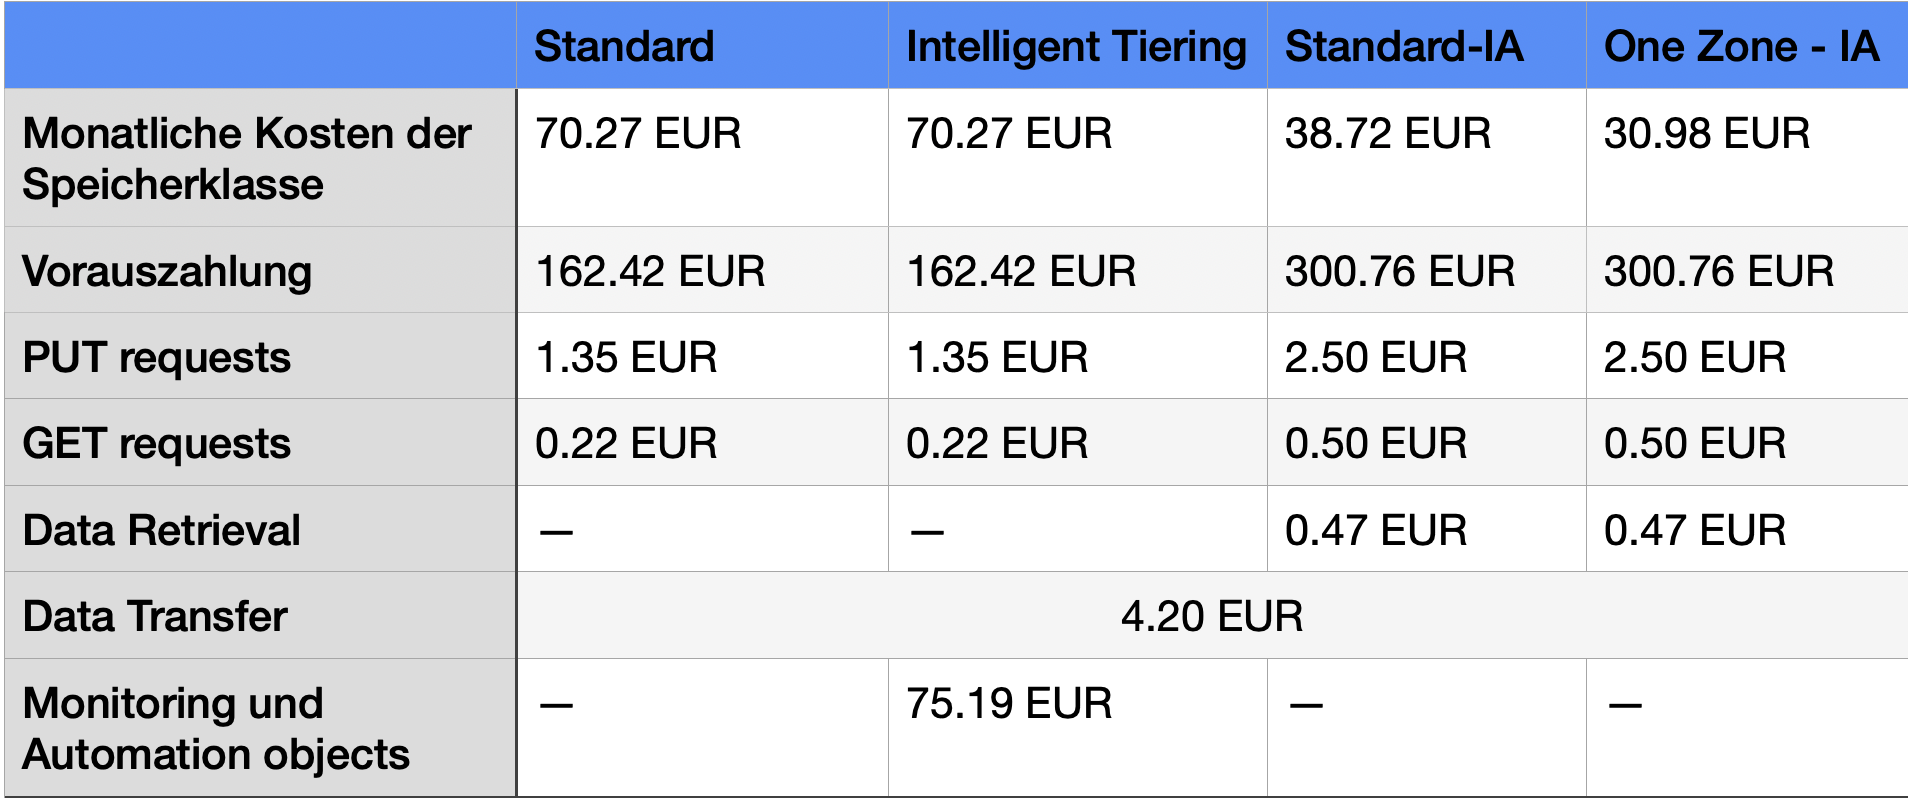
\includegraphics[width=12cm,keepaspectratio]{Pictures/AWSKostenOhneGesamt.png}
\caption{Gesamtkosten der Datenspeicherung in Amazon S3}	
\end{figure}

Zuerst werden die Einheitsumwandlungen durchgeführt. Dabei werden die angegebenen 3TB im Monat mal die 1024GB multipliziert, um die exakte Menge an GB auszurechnen. Dies ist bei 3072GB. Danach wird die Objektgröße von 400kb in GB umgerechnet, was 0.000095367432 GB ergibt. Anschließend werden die Preise kalkuliert. 

\newpage

\begin{align}
	\frac{3072 \text{ GB per Month}}{0.000381469728 \text{ GB average item size}} = 8.053.064 \text{ number of objects}\\
	3072 \text{ GB} \times 0.0135 \text{ USD} = \text{41.472 USD Standard-IA costs}\\
	67.000 \text{ PUT requests} \times 0.00001 \text{ USD per request} = 0.67 \text{ USD (PUT requests cost)}\\
	134.000 \text{ GET requests} \times 0.000001 \text{ USD per request} = 0.134 \text{ USD (GET requests cost)}\\
	50 \text{ GB} \times 0.01 \text{ USD} = 0.50 \text{ USD (data retrievals cost)}\\
	41.472 \text{ USD} + 0.67 \text{ USD} + 0.134 \text{ USD} + 0.50 \text{ USD} = \underline{\textbf{42.78  USD (Total Standard-IA)}}\\
	8.053.064 \text{ number of objects} \times 0.00001 \text{ USD} \\ = \text{80.53 USD (Cost for PUT, COPY, POST requests for initial data)}
\end{align}

Die obigen Formeln sind ähnlich wie bei der Standard und One Zone-IA, wenn man dabei die jeweiligen Gebühren aus dem Kosten Abschnitt übernimmt. Bei der Intelligent Tiering gibt es noch den Unterschied, dass die Kosten für Monitoring und Automation dazu kommt und die Einteilung des Speichers in Prozent auf drei Speicherklassen. In der letzten Zeile der abgebildeten Tabelle werden die Gesamtkosten gemeinsam mit den Kosten des Datentransfers, Vorauszahlung und die puren monatlichen Speicherkosten der jeweiligen Speicherklassen addiert.\\

\textbf{Google Cloud Storage}\\

In der folgenden Tabelle werden die Kosten von Google Cloud Storage für drei Speicherklassen zusammengefasst:

\begin{figure}[h]
\centering
	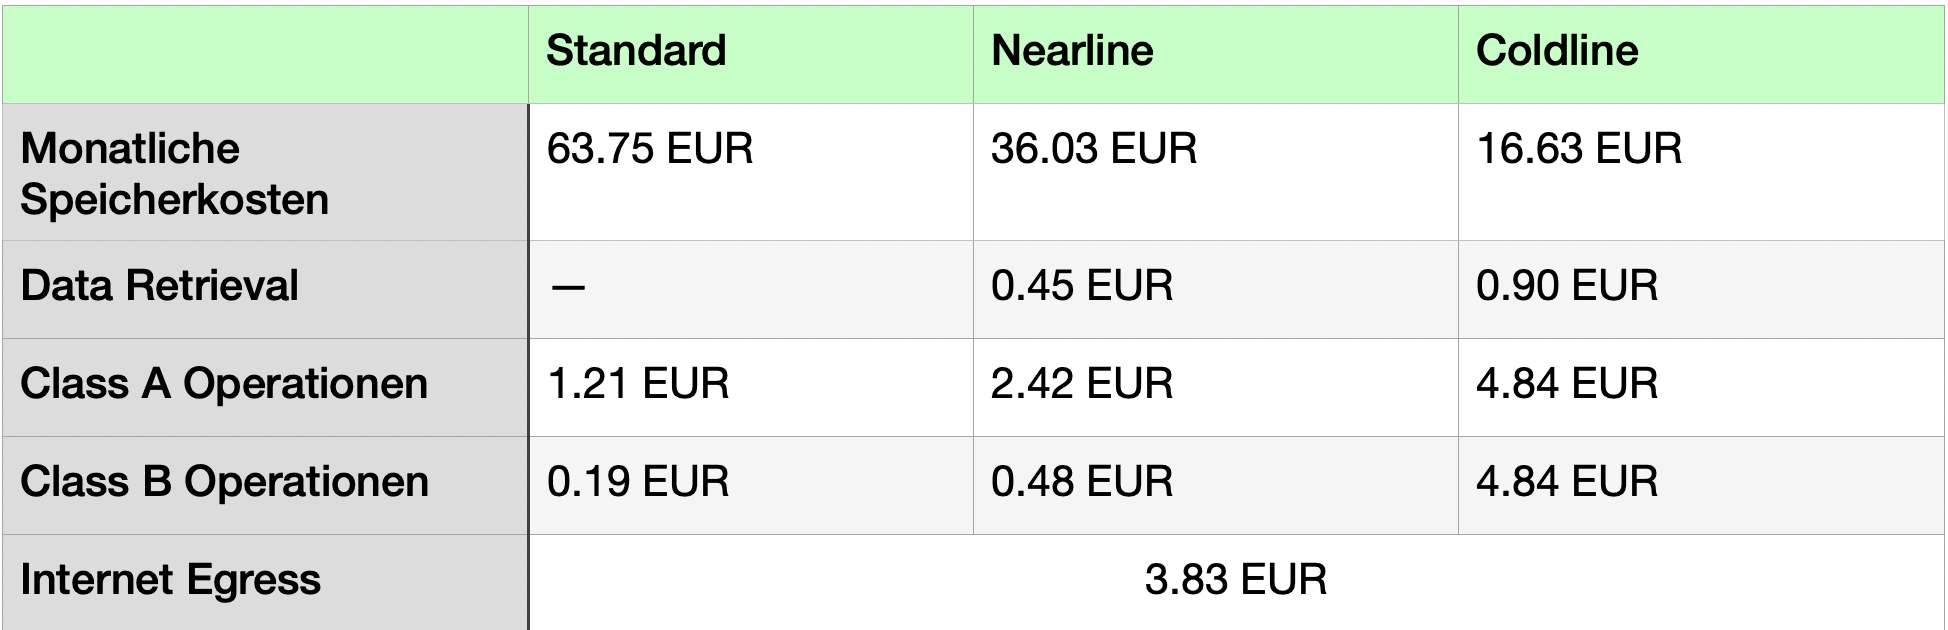
\includegraphics[width=12cm,keepaspectratio]{Pictures/GCKostenOhneGesamt.png}
	\caption{Gesamtkosten der Datenspeicherung in Google Cloud Storage}
\end{figure}

Die teuerste Speicherklasse mit 64.10 Euro ist die Standard Klasse. Die billigste mit 16.63 Euro ist die Coldline Klasse. Die Nearline Speicherklasse ist mit 36.03 Euro teurer als die Coldline. Bei der Standard Klasse gibt es keine Gebühren für die Daten Retrieval.

\newpage

\subsection{Performance Analyse}

In diesem Abschnitt erfolgt die Messung der Performance für die Dienste von AWS und Google Cloud. Dabei werden 2300 Dateien sowohl für den Upload als auch für den Download betrachtet. Die Anzahl der Dateien ergibt sich aus der monatlichen Gesamtanzahl von 67 000 Objekten, die durch 30 Tage geteilt wird. Um eine realistische Performance-Analyse durchzuführen, bieten beide Cloud-Anbieter verschiedene Diagnose-Tools an, die während der Arbeitszeit eingesetzt und gemessen werden. Dadurch wird eine praxisnahe Bewertung der Performance ermöglicht.\\

\textbf{AWS}\\

AWS bietet Dienste für die Performance Analyse. Unter anderem die Amazon CloudWatch, S3 Storage Lens und die S3 Transfer Acceleration. Die AWS CLI stellt einfache Methoden zum S3 Upload und Download Tests vor. Beispielsweise kann man mit dem Befehl:

\begin{code} aws s3 cp \end{code}

Dateien hoch,-und herunterladen und die Zeit für die benötigte Request verwenden. Auch mit der AWS SDK können Performance Test Skripte geschrieben werden. Diese Methode wird für den Prototypen angewendet. Dabei werden Tests bereitgestellt, die mehrere Dateien automatisch hoch, und herunterlädt und dabei die Zeit misst, die vergangen ist. 

\newpage

\textbf{Google Cloud Storage}\\

GC bietet einen eigenen "gsutil" Tool für die Performance Analyse. Im Abschnitt Performance bereits erwähnt können durch die perfdiag Funktion Performance Diagnosen erstellt werden. 

\begin{quote}
	Mehrere Testdateien werden aus einem angegebenen Bucket hoch-und heruntergeladen. Nach der Analyse werden alle Testdateien wieder gelöscht nach erfolgreicher Diagnose. Die gsutil Performance kann von einigen Fakoren beeinflusst werden wie vom Client, Server oder Netzwerk. Möglich sind die CPU Geschwindigkeit, der verfügbare Speicher, die Netzwerk Bandbreite, Firewalls und Fehlerraten zwischen gsutil und den Google Servern. Die perfiag Funktion wurde dafür bereitgestellt, damit Nutzer Messungen durchführen können, die beim Troubleshooting von Performance Problemen helfen, vgl. \cite{gc-perfdiag}.
\end{quote}

Um die Performance Diagnose auszuführen, kann der folgende Befehl verwendet werden:

\begin{code} gsutil perfdiag -o test.json -n 67000 -s 400kb gs://leoticket-bucket \end{code}

Die -o Option schreibt den Output des Ergebnisses in eine Datei. Die Output Datei ist eine JSON Datei mit System Informationen und enthält die Performance Diagnose Ergebnisse. Die -n Option setzt die Anzahl der Objekte, die heruntergeladen und hochgeladen werden sollen während dem Test. Mit der -s Option kann man die Objektgröße in bytes angeben. Zum Schluss wird der Name des Buckets angegeben. Damit der Befehl erfolgreich ausgeführt werden kann, braucht man die entsprechenden Rechte und muss sich authentifizieren können. Um die Performance auf leoticket zu analysieren, werden 9000 Objekte mit jeweils 100kb Objektgröße verwendet. Diese Daten stammen aus dem Kosten Abschnitt. Anschließend wird die Performance über die SDK von Cloud Storage ähnlich wie bei AWS getestet. 

\newpage